\section{Literature Survey}
The purpose of this literature survey is to provide the reader with a frame of reference from which they can understand the motivation, design choices, and the overall scope of this project. We begin with informal definitions of several key concepts which will be encountered in this report. A brief history of computing systems, and the design of the 8086 microprocessor and the original IBM PC are discussed. We conclude this literature survey with a brief discussion of the deficiencies of the current engineering and technical education in India.

\subsection{Algorithms and Programs}
The definition of computer has gone a several changes throughout history. Before 1950's, the term usually referred to a person who had the job to do calculations or \textit{computations} \cite{evans2020broad}. Nowadays, it refers to a machine which processes data according to instructions fed into it. Majority of such machines are made out of electronic components and work on the principles of digital logic. Therefore, by the term computer one implicitly refers to a \textit{digital electronic computing system} \cite{ionescu2015categories}.  One common denominator throughout this transformation of computing systems has been that they need to be told to perform a particular task. The task to be performed is usually divided into smaller, manageable tasks or instructions. A sequence of such tasks is called an \textit{algorithm}. Each sub-task which makes up an algorithm is called a \textit{step} or an \textit{instruction}. Algorithms are usually written in a human language or mathematical symbols or, in general, both.\\
A good algorithm has five important features \cite{knuth1997art}:
\begin{enumerate}
\item \textit{Finiteness}: It must stop after a finite number of steps.
\item \textit{Definiteness}: Each step of the algorithm must be precisely defined.
\item \textit{Input}: An algorithm should have zero or more inputs.
\item \textit{Output}: An algorithm should have one or more outputs.
\item \textit{Effectiveness}: An algorithm is said to be effective if, in principle, if each of its steps can be executed manually, using pencil and paper, in a finite length of time.
\end{enumerate}
A simple example at this point would be helpful. Consider a student who is given the task to print out whether a given number is prime or not. He will first begin by defining prime numbers.\\
\textbf{Definition:} A number is said to be prime if it is only divisible by 1 and the number itself.\\
With this definition at hand, it becomes obvious that to test whether a number $N$ is prime or not, we have to check whether it is divisible by any other natural number except for 1 and itself. Upon inspection the student might observe that one does not need to test $N$'s divisibility with numbers greater than $N / 2$. The final algorithm that is obtained is:
\begin{steps}[leftmargin=2cm]
\item $n = 2$, $N = 0$.
\item Input $N$.
\item If $n > N/2$, then jump to step 6. 
\item If $N$ is divisible by $n$, then jump to step 7.
\item If $N$ is not divisible $n$, then $n = n + 1$ and jump to step 3.
\item Print \verb|N is a prime number| and end program.
\item Print \verb|N is not a prime number| and end program.
\end{steps}
A modern digital computer would not be able to understand these commands. It can only understand and execute instructions native to its architecture. A program consisting of opcodes of instructions and data, all in binary/hexadecimal format, is called \textit{machine code}. A file consisting of machine code is called a \textit{binary file} or, simply, \textit{binary}. A computer is able to understand only binaries and executes them in one shot (provided they mean something. Not every hexadecimal number can be mapped to an opcode). However, implementing any algorithm in machine code would take a significant amount of time. Debugging the binary would be even more troublesome. 
The problem can be solved by defining a language which satisfies the following criteria:
\begin{enumerate}
\item After sufficient training, a human being should be able to implement and debug algorithms in this language.
\item The algorithm implemented in this language can be easily converted into a binary using some conversion tool.
\end{enumerate}
A language satisfying both of these criteria is called a \textit{programming language}. The act of writing code in a programming language is called \textit{programming} or \textit{coding}. An algorithm implemented in such a language is called a \textit{program} or \textit{code}.\\
The simplest kind programming language is \textit{assembly language} (One can call machine code as a programming language, however, it is no longer used directly to practically program any computer). In assembly language, every instruction and register, instead of being referred by their opcode, are referred by a mnemonic. Labels are used to mark locations instead of hardcoded addresses. An \textit{assembler} is used to convert these mnemonics and labels into machine code.\\
While learning assembly language is not impossible, it has, however, a very steep learning curve. This calls the need for \textit{higher level languages} (HLL). These programming languages mask the programmer from the architecture of the machine they are working on. This enables them to direct their energies towards developing and implementing algorithm to get the task done. Every HLLs have its own set of symbols for defining operations and data structures, and semantics and syntax for successfully implementing algorithms \cite{hthreads2006glossary}\cite{chu1975concepts}. C is one such programming language. The algorithm for testing whether a number is prime or not can be implemented in it.
\begin{Verbatim}[tabsize=8]
#include <stdio.h>
#include <stdlib.h>

int main(int argc, char ** argv)
{
	int n = 2, N = 0;
	fscanf(stdin, "%d", &N);
	for (; n <= N / 2; ++ n) {
		if (N % n == 0) {
			fprintf(stdout, "N is not a prime number\n");
			exit(0);
		}
	}
	fprintf(stdout, "N is a prime number\n");
	return 0;
}
\end{Verbatim}
A C \textit{compiler} takes this \textit{source file}, checks it for errors, and if none are found, converts it into its equivalent assembly code. The assembler takes this assembly source file and converts it into an \textit{object file}. An object file contains machine code (binaries), but is not yet in machine executable form as addresses of labels and library functions have not yet been included into it. An object file has a code section and data section (besides other sections depending upon the object file format being used). Machine code of instructions corresponding to a single statement of C code are kept in the code section, whereas symbols/variables like \verb|n| and \verb|N| in the above code are placed in the data section. Finally, the object file is passed to another program called \textit{linker} which resolves the addresses of various symbols used, includes the library functions' binaries and produces an executable binary file.\\ 
Problems, algorithms and their implementations in a programming language get more interesting and complex than the simple example that has been provided here. As the size of a program increases, it is often wise to split it into several source files, each of which is individually compiled, and the resulting object files are linked to produce a single binary. \autoref{fig:stepcompile} shows the the compiling, assembling, and linking of programs with multiple source files.
\begin{figure}[h]
\centering
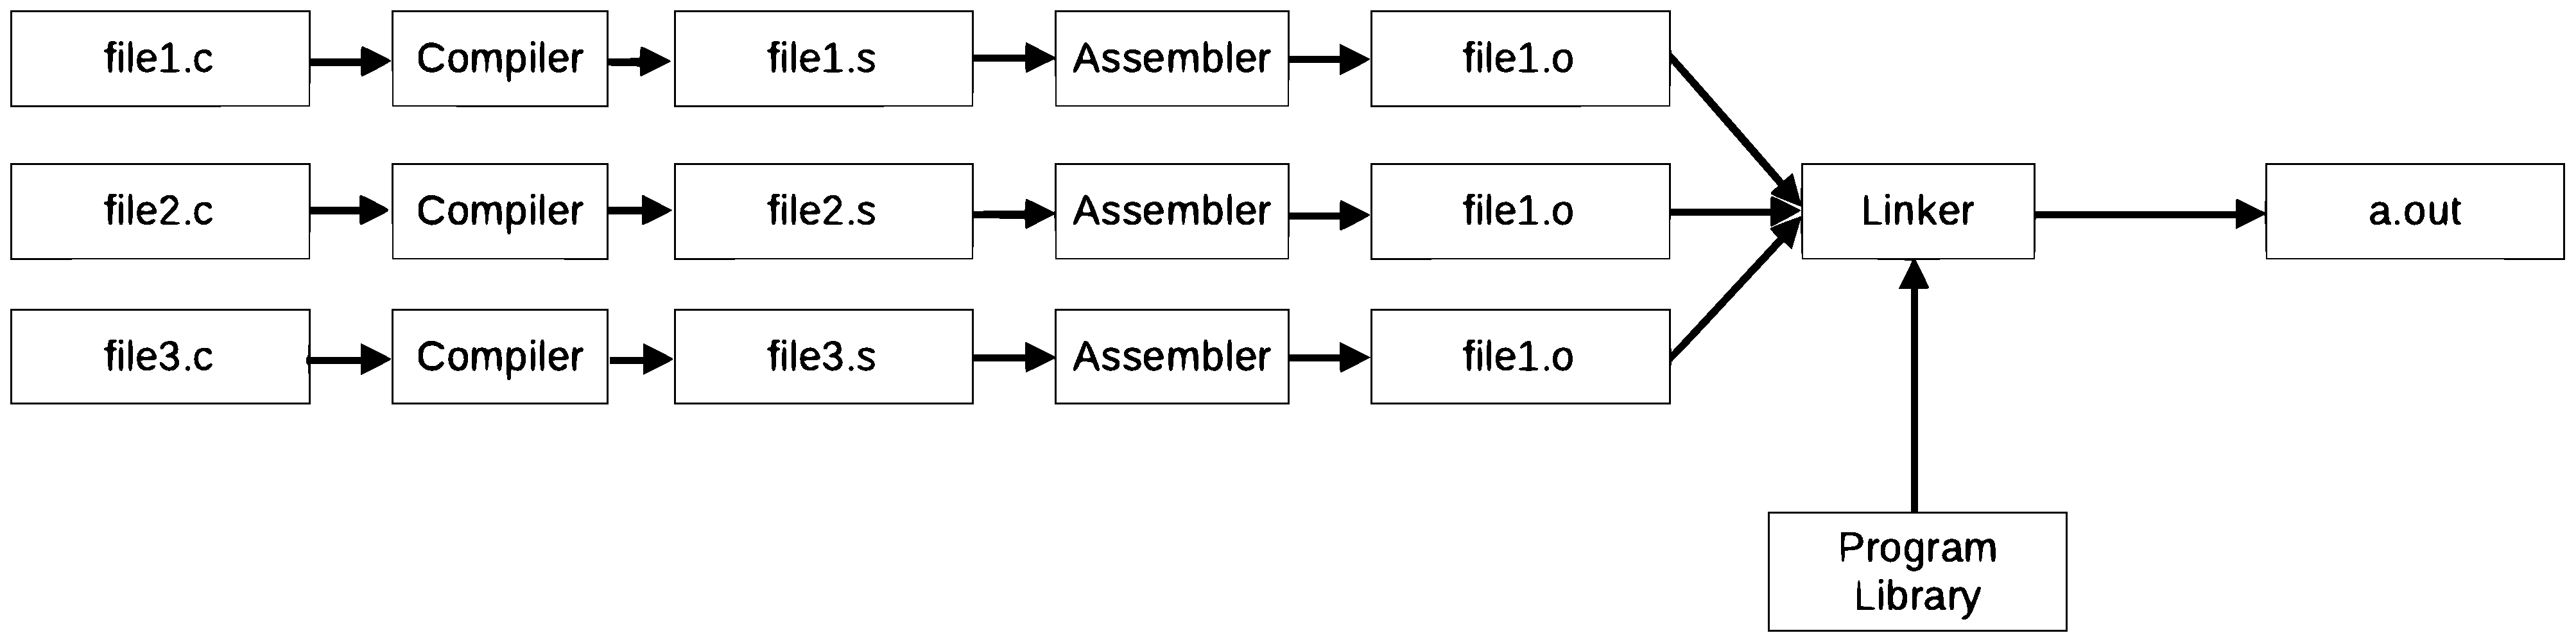
\includegraphics[scale=0.22]{figures/steps-of-compilation.eps}
\caption{Steps involved in building a C program having multiple source files}
\label{fig:stepcompile}
\end{figure}

\subsection{Operating Systems}
\subsubsection{What is an Operating System?}
Generally a computer is running multiple tasks at a time. This increases the complexity of building binaries of each individual program and running them. The complexity of running multiple tasks at the same time can be understood by two examples.\\
\textbf{Example 1:} Take the case of a student taking a numerical methods exam. Generally, questions in numerical methods require us to perform certain operations repeatedly till the answer starts converging satisfactorily. The student will be required to perform such computations many times. He must make sure that his scratch-pad is neat so that the results of different iterations and questions do not get mixed up. He must also make sure that the scratch-pad is utilized efficiently, lest he will run out of space to perform more computations.\\
\textbf{Example 2:} A librarian is tasked with managing a library. This task is composed of several tasks, for example, issuing a book as per member's demand, making sure that all books are in their specific section, etc. These tasks require that the librarian create and maintain a record of every member and every piece of literature which is present in the library.\\
In each of these examples, a single human computer was given several tasks to perform which can be performed only if every individual task is dealt with without affecting other tasks. In a computer, we run multiple tasks/programs at the same time. An editor allows us to edit source files, a shell allows us to run the compiler and a linker, a document viewer allows us to read manuals, and so on. It has to be made sure that no two programs interfere with each other. As programs often acts on files, a \textit{filesystem} also needs to be in place to make sure that the files are operated on correctly. The program tasked with managing the resources of the computer and providing an environment in which programs can run is the \textit{operating system} \cite{tannenbaum2003operating}.\\
Without an operating system, all sorts of chaos can happen. A program can start interpreting the code section of another as data, and overwrite it completely. Two or more programs accessing the printer without any prioritization and buffering will result in parts of text outputted by each program getting printed. Thus, an operating system can be thought of as the crucial software responsible for maintaining order and preventing possible chaos.

\subsubsection{System and Application Software}
Certain application-independent programs like shell, editor, compilers, windowing system, etc. are shipped along with the operating system. These are called \textit{system software}. Software like web browser, games, word processors, etc. are called \textit{application software}. System software provides the environment in which application software can run. Continuing with the analogies provided in the previous two examples, if the student is to be considered as an operating system which is managing everything, then the sheet of paper and the pen he uses are the system software. The equations he scrolls are the application software. He could have scrolled them out on the furniture, or on the walls, but he uses the tools he is provided with to get the job done. Similarly, if the librarian is an operating system, then the chairs and lights in the library are analogous to system software. Members can be made to sit on the floor and read; they are simply using the tools they are provided. Clearly, while one can choose between the shell, compiler, or the window manager they wish to use, the user is not free to write their own scheduler \citep{tannenbaum2003operating}. \autoref{fig:compsyslayout} shows the arrangement of hardware and software in a typical computer.
\begin{figure}[h]
\centering
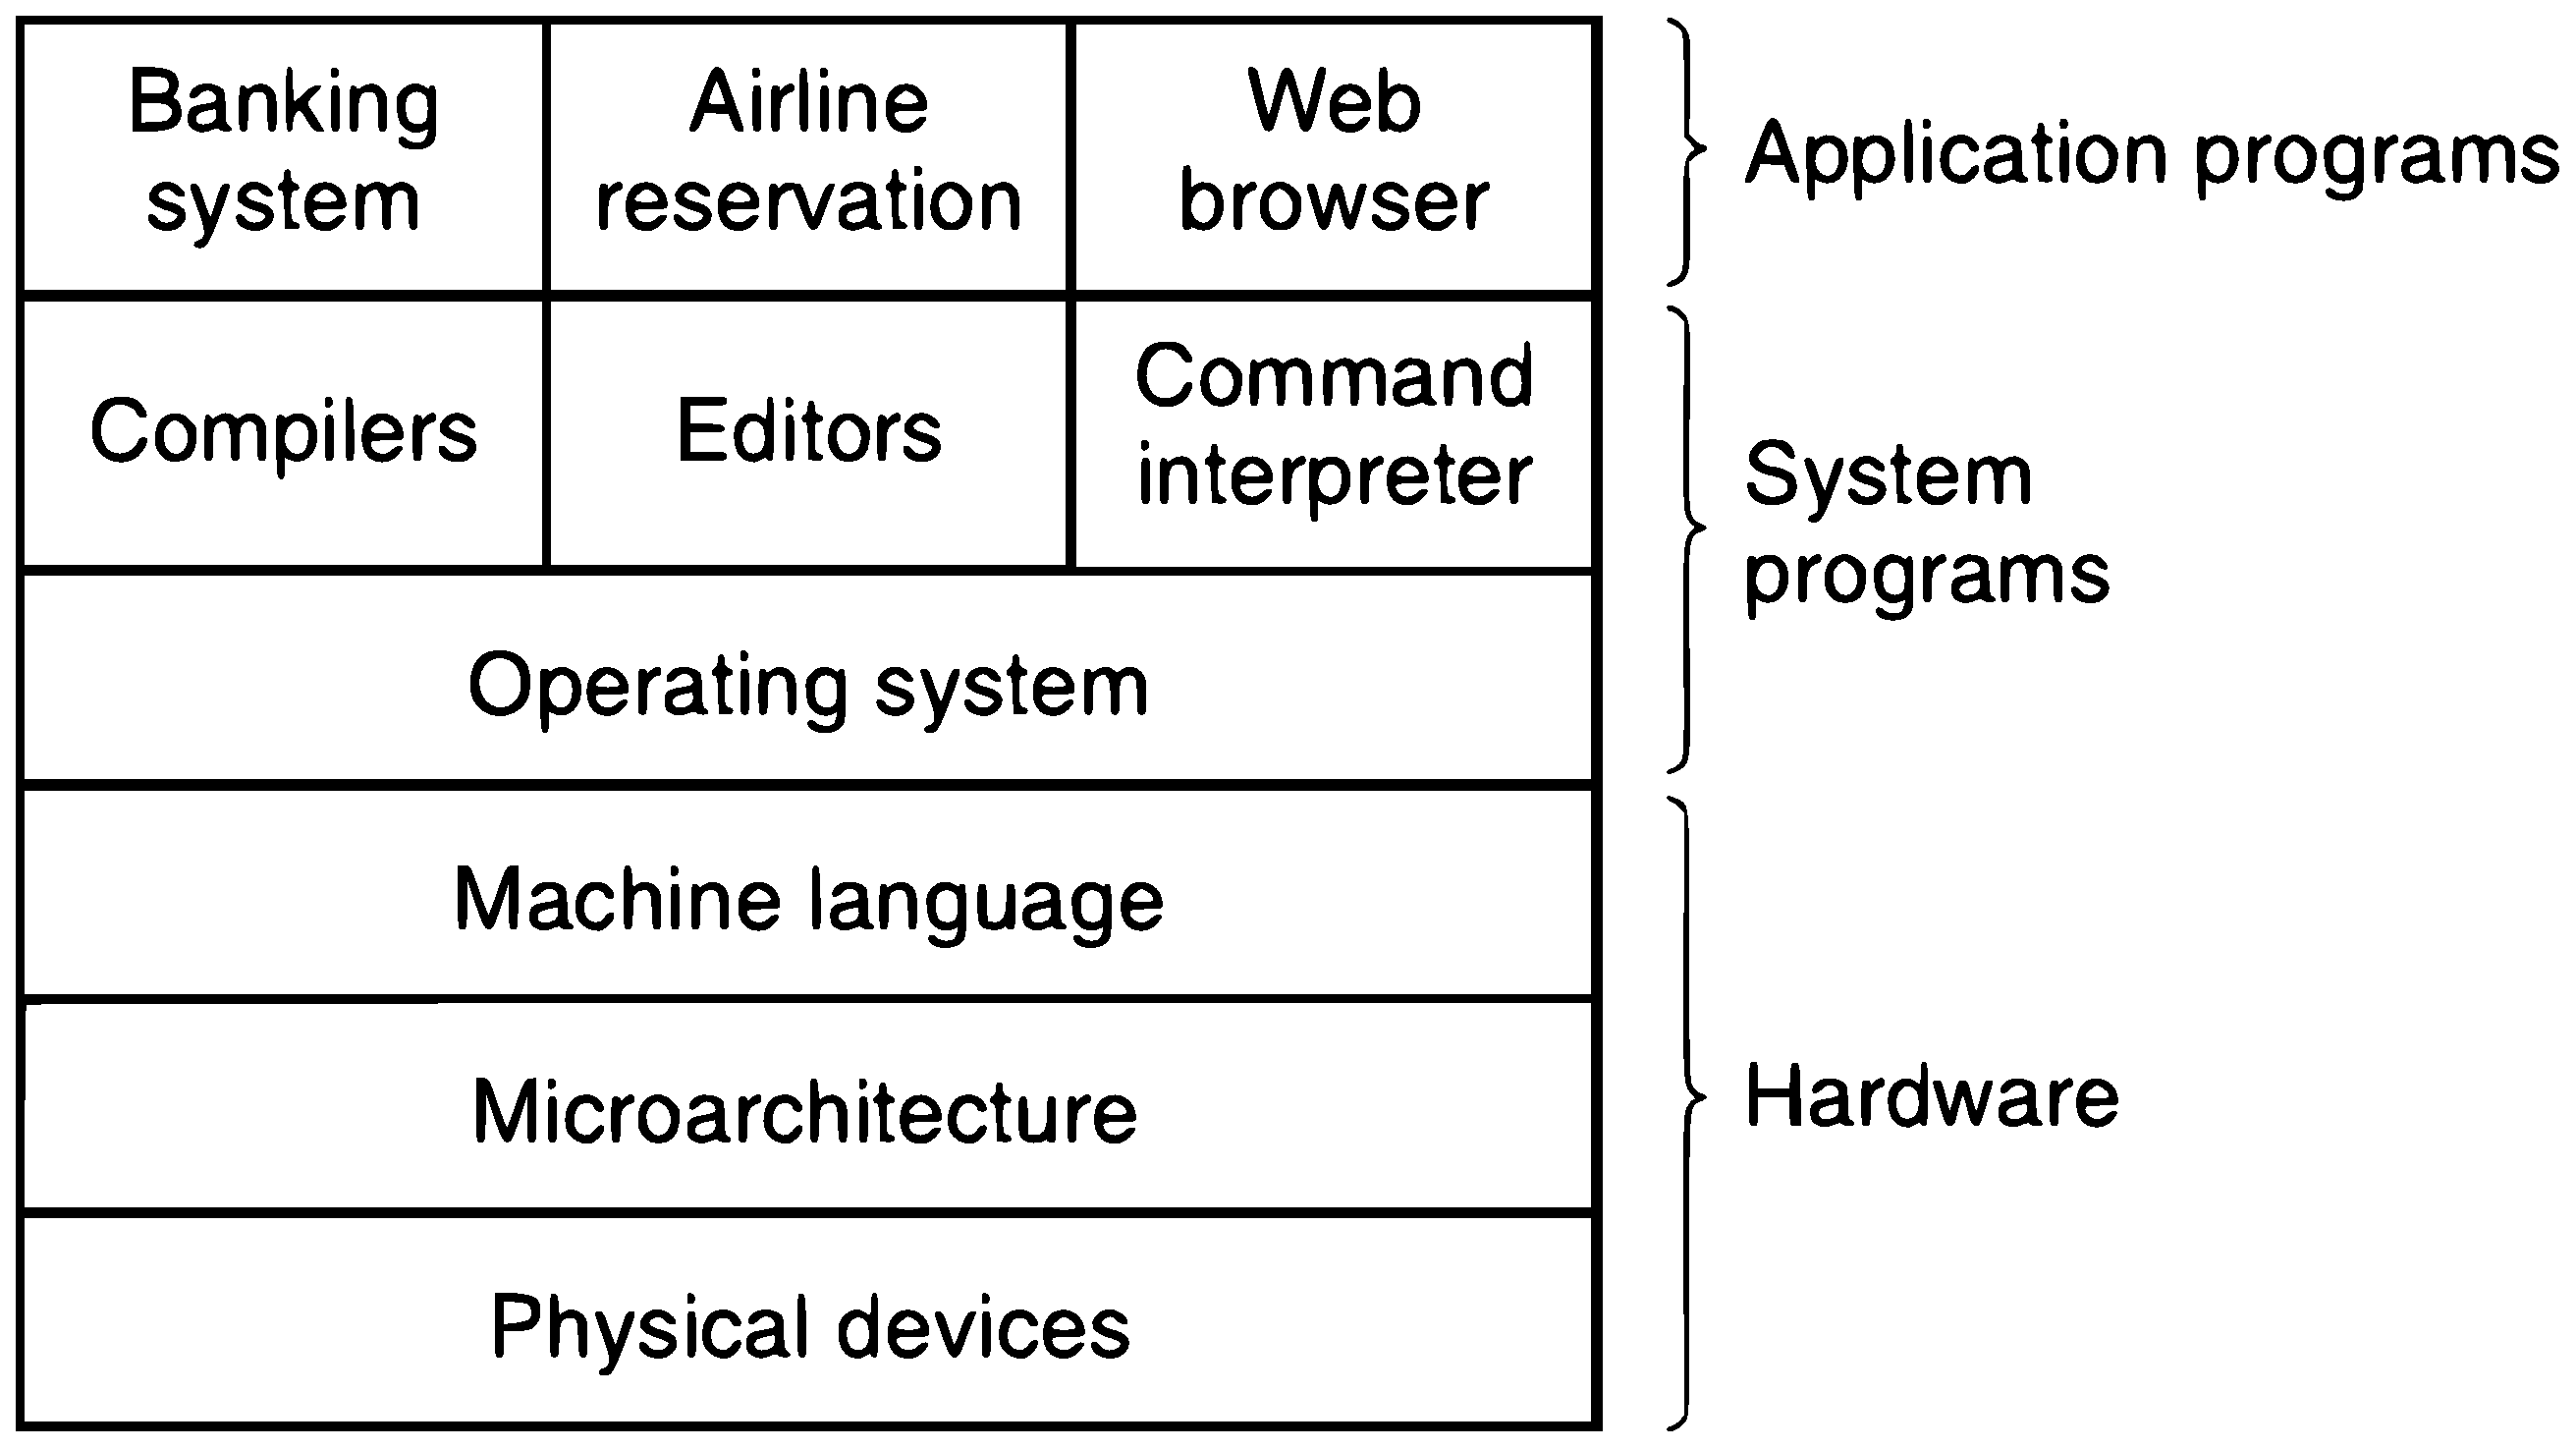
\includegraphics[scale=0.22]{figures/comp_sys_layout.eps}
\caption{Layout of a typical computer system \cite{tannenbaum2003operating}}
\label{fig:compsyslayout}
\end{figure}

\subsubsection{Functions of an Operating System}
We have described what an operating system is with the help of analogies. These analogies showed us that in operating system is the software which is responsible for managing the resources of the system. As a resource manager, the operating system has to make sure that programs do not interfere with each other. As most of the operating system today support multiple users, it becomes important that the resources allocated to each user are managed carefully. This becomes important in large organizations like universities and industries, where multiple computers are connected to a single server. This type of resource management involves sharing of resources or \textit{multiplexing}. There are two types of multiplexing: time multiplexing and space multiplexing. Time multiplexing involves allocating a specific a unit of time for each program to use the CPU. It also involves accessing I/O devices based on priority by various programs.  Space multiplexing involves giving each user (or a program) a part of the resource. An example would be the storing of all programs in main memory. This way, they can easily be time multiplexed to use the CPU and memory is not entirely given to one program only. Secondary memory like hard disks are also space multiplexed by giving each user some disk space in which they can store and organize their files.\\
Operating systems also perform the function of extending the capabilities of the machine so as to make it pleasant to deal with. When a programmer, or an ordinary user use a computer, they should be only considered with getting their job done. They should not have worry implementing a driver for hard disk, monitor, and other peripherals. Operating systems extend the instruction set of the machine by providing utility functions which allow a programmer to easily use the resources of the computer. The most fundamental utility functions are called \textit{system calls}. Examples would be \verb|read| and \verb|write| system calls in UNIX-like operating systems. These system calls are used by programs to access and operate on various files and peripherals like the screen. By providing the programmer with system calls and by setting up an environment in which work can easily be done, operating system extend the capabilities of the machine. One can say that operating systems provide the user with a virtual machines which is easier to deal with \cite{tannenbaum2003operating}.  

\subsection{A Brief History of Computers, Programming Languages, and Operating Systems}
Knowing about the history of computers is important for several reasons. Tannenbaum \cite{tannenbaum2003operating} explained the importance of learning about old systems with the example of contiguous memory allocation:
\begin{quotation}
\textit{...history may repeat itself in computer science as new generations of technology occur. Contiguous allocation was actually used on magnetic disk file systems years ago due to its simplicity and high performance (user friendliness did not count for much then). Then the idea was dropped due to the nuisance of having to specify final file size at file creation time. But with the advent of CD-ROMs, DVDs, and other write-once optical media, suddenly contiguous files are a good idea again. For such media, contiguous allocation is feasible and, in fact, widely used. Here all the file sizes are known in advance and will never change during subsequent use of the CD-ROM file system. It is thus important to study old systems and ideas that were conceptually clean and simple because they may be applicable to future systems in surprising ways.}
\end{quotation}
A lesson in the history also allows a person to understand the reason behind the design of present computers. For example, after reading the design of DEC's PDP-11, it can be seen how it influenced the design of x86 family of processors \cite{supnik2004simulators}.\\
History of computers involve studying their evolution. Just like a study of human history consists of the study of various civilizations and generations,  a study of computer history involves the study of various generations of computers. Beginning of a new generation are marked with the usage of newer, better, and reliable technology in comparison to the previous generation. The technology most  used for this classification is the hardware. By using hardware as the basis for classification, most authors divide computer history into five generations, starting in 1951 with the launch of UNIVAC I \citep{ionescu2015categories}. The \autoref{table:compgen1} is an excerpt from one such detailed table giving the history of computers \cite{friedman1992babbage}. 
\begin{table}[H]
\caption{Generations of Computers on the Basis of their Hardware}\label{table:compgen1}
\begin{center}
\begin{adjustbox}{width=1.0\textwidth,center=\textwidth}
\begin{tabular}{|c|c|c|c|}
\hline
\textbf{Generation} & \textbf{Year} & \textbf{Technological Features} & \textbf{Examples}\\
\hline
1st Generation & 1951-1960 & Vacuum tubes & UNIVAC I, IBM 650\\
\hline
2nd Generation & 1959-1965 & Transistors & IBM 1401, IBM 7094\\
\hline
3rd Generation & 1964-present & Integrated circuits & IBM 360, PDP-11 (16-bit minicomputer)\\
\hline
4th Generation & 1971-present & VLSI, Microprocessors & Altair 8800, Commodore VIC-20\\
\hline
5th Generation & Present-future & Parallel processing architecture & Computers using Pentium or higher\\
\hline
\end{tabular}
\end{adjustbox}
\end{center}
\end{table}
By using programming languages and operating systems as the basis for classification, we arrive at similar results \cite{tannenbaum2003operating}. This type of classification is more useful in context of the present report and, therefore, it will be discussed from here on.

\subsubsection{The Zero Generation Computers (1645--1945)}
This generation of computers came before the invention of digital computers. In reality, if one takes into consideration human computers and mechanical calculators, then computers have been around since eternity. The oldest known mechanical computer would be the Antikythera mechanism from 87 BC which was supposedly used to predict astronomical positions and eclipses \cite{ionescu2015categories}\cite{10.1115/1.2018-SEP1}. More examples of early calculators would be abacuses and slide rules, the latter being used well into the 1970's and is credited for putting the man on the Moon \cite{stoll2006slide}. \\
The first mechanical calculator would be Pascal's calculator (or Pascaline). It was capable of addition and subtraction, and multiplication and division using repeated addition and subtraction, respectively \cite{chapman1942pascal}.\\ 
The most significant mechanical computers were Charles Babbage's difference engine and analytical engine. Construction of the difference engine began in 1819 and a small portion of it was completed and demonstrated in 1822. The difference engine used the method of finite differences to interpolate functions \cite{dasgupta2014began}. The analytical engine was a more complex machine which introduced several new concepts like program and memory. Although not completed during Babbage's lifetime, the analytical engine was shown to be programmable by Ada Lovelace \cite{tannenbaum2003operating}.\\
Mechanical differential analyzer's and their analog counterparts used during the two world wars were also programmable. The integrators and differentiators they were made up of were linked together to model systems through their differential equations. The output was a plot of the system's output with respect to input. As signals out of blocks were feeble, they were passed through an amplifier before being passed to the next block. Each of these amplifications were to be taken into account when interpreting the output \cite{robinson_t_2005_918318}.\\
For each of these mechanical computers, the concept of a program was plugboard wiring or positions of mechanical linkages. The concept of an operating system, or even programming languages, didn't exist yet.

\subsubsection{The First Generation Computers (1945--1955)}
Work on developing mechanical digital computers continued until 1945. These early calculating engines were made up of relays, which were later replaced by much faster vacuum tubes. One of the most remarkable person involved with the first generation computers was Konrad Zuse. In 1936, he completed a relay based mechanical computer named \textit{Z1} in his parent's basement. It was a floating point mechanical calculator which could be programmed using perforated 35 mm films. Later, he designed Z2 and Z3, the latter having 2600 relays, 22-bit word length and operated at frequency of 5-10 Hz \cite{morelli2001dalle}. While working on Z4, he found that programming on machine code was hard. He then designed the world's first high-level language named \textit{Plankalkül} \cite{hellige2013geschichten}.\\
Meanwhile in United States, J. Presper Eckert and John Mauchly invented the ENIAC (Electronic Numerical Integrator and Comparator) at the University of Pennsylvania in 1945. It was the first general-purpose programmable digital computer. Both the hardware and software of the ENIAC was different from modern computers. It was made up different machines each capable of performing a specific arithmetic operation. It was programmed by wiring a plugboard and three portable function tables. Each function table had 1200 ten-way switches which were used to enter a table of numbers. Programming was done only by the members of the ENIAC team after the program has been thoroughly tested \cite{cruz2013eniac}. In 1996, on the 50th anniversary of the ENIAC, using CMOS technology, a 7.4 mm x 5.3 mm chip with the same functionality as the ENIAC was successfully built \cite{6302808}.\\
EDVAC (Electronic Discrete Variable Automatic Computer), ENIAC's successor, was also designed by Eckert and Mauchly before ENIAC got completed. It was put into operation in 1951. Eckert and Mauchly, and the design team of the EDVAC were joined by the famous mathematician John von Neumann who acted as a consultant. Neumann later wrote a 101 page incomplete monograph titled \textit{The First Draft of a Report on the EDVAC} \cite{von1993first}. In it he described a computer architecture in which program and data are stored in the same memory space. This architecture is called the \textit{von Neumann architecture}. A machine using this architecture is called a \textit{stored program} machine. The first computer to implement von Neumann architecture was the EDSAC at Cambridge. A computer architecture having program and memory in different memory spaces is called the \textit{Harvard architecture}.\\ 
It was soon realized that programming computers in machine code by interlinking various arithmetic and logic blocks using a plugboard/control panel was inefficient. Computers produced near the end of this generation had, besides a plugboard, a punch card input-output unit. User, using a modified typewriter, punched holes into cards. These cards were fed into a card reader. The card reader read the cards using optical sensors: light shown on the cards passed through the punches and activated the optical sensor below them. This was interpreted as the binary '1'. The rest of the optical sensors registered a binary '0'. The resulting binary was fed into the main memory of the computer, usually a magnetic drum. Results were punched out on the cards using an opposite mechanism.\\
An example of a machine which was operated this way was the IBM 650. The IBM 650 was a stored program machine. It had console from which the machine could be programmed in machine code using octal switches and its state during program execution could be seen. Data was written and read from its magnetic drum memory by the IBM 533 input-output unit using punched cards \cite{andree1958programming}. Donald Knuth dedicated his magnus opus \textit{The Art of Computer Programming} to an IBM 650 which he used to learn programming while an undergraduate at the Case Institute of Technology \cite{knuth1997art}.
It should be noted that besides the complexity of programming these early computers, the task of debugging a program and fixing the machine was also hard. Considerable time was lost in finding the vacuum tube which has burned out.

\subsubsection{The Second Generation Computers (1955--1965)}
Invention of the transistor in 1947 ushered a new era in the field of electronics and computer science. Vacuum tubes were replaced by transistors to build amplifiers and digital logic circuits. The small size and high power efficiency of transistors meant that computers, instead of requiring a hall to be fit into, could now be fit into a room. As the reliability of transistors was high in comparison to vacuum tubes, it meant that computers made using them could easily be mass produced and sold without the customers worrying about repairs for a long time. Computers of this generation were called \textit{mainframes} \cite{tannenbaum2003operating}. Two important examples of mainframes from this generation would be the IBM 1401 and 7094 computers.\\
Around this same time, assembly language gained prominence and high-level languages like COBOL and FORTRAN were introduced. Assembly language is still used today to develop firmware (BIOS, embedded system software). Time critical parts of software used in aeroplanes, fighter-jets, rockets, etc. are still written in assembly language. Inline assembly code can be found in the source code of the Linux kernel. FORTRAN is also still used  for scientific calculations in experimental physics and other applied technical domains. It has been called the "mother tongue of scientific computing" \cite{halpern1993large}. COBOL, on the other hand, is a nearly obsolete language: these days COBOL programs can only be found in mainframes in various business firms. They haven't been replaced by programs written in other languages because the cost of replacing a known technology which has been working reliably for the past five decades is very risky \cite{mitchell2006cobol}.\\ 
To program these computers, a programmer would first write the program on paper in either assembly language or FORTRAN. Then, he would type it out on a machine like the IBM 029, which would encode each keystroke on the typewriter by punching the cards. In the end, the programmer would be having a deck of cards having his program. This deck was fed into a card reader connected to the computer. Here, the deck was read and the program was stored in the main memory of the computer. The computer then executed the program and the results were stored in its main memory. To print out the results, a printer would read the memory and print the output on a roll of paper. The next deck of cards containing another program/job was then loaded and executed by the computer.\\
It should be noted that while the cards were being read and the results were being printed, the computer was sitting idle. That is, it was doing no data processing during the time it was reading decks, copying them to memory, or printing data from memory. To reduce this waste of time, \textit{batch system} was invented. In it, an expensive computer like the 7094 which was good at numerical calculations was were used solely for executing programs. The task of card reading and writing was relegated to computers like the 1401 which were good at reading cards to tape, copying data and reading tape. A collection of decks, each containing different jobs/programs, was called a batch. It was fed into a 1401 which copied the programs in the batch to a magnetic tape. An operator would then take this tape and connect it to the tape drive of the 7094. The 7094 then ran a special program which would read each program on the first tape one-by-one and write their output to a second tape instead of printing them out. This program was a precursor to modern operating systems. When a batch of job had been executed, the second tape was taken by an operator who would connect it to the tape drive of the 1401. Its contents were read and printed on a roll of paper. Meanwhile, another operator would connect a tape containing another batch of job to the tape drive of the 7094 \cite{tannenbaum2003operating}.

\subsubsection{The Third Generation Computers (1965--1980)}
Miniaturization of computers continued with the introduction of integrated circuits (ICs). The first monolithic IC was invented by Robert Noyce in 1959. The first prominent use of integrated circuits was made in the construction of the Apollo Guidance Computer (AGC). Consultants hired by NASA mathematically proved that a computer made using ICs, transistors, and diodes would have a very high probability of failure. Their calculations used the assumed failure rate of these components. Eventually, Eldon C. Hall, leader of the hardware designing team for the AGC at MIT and an advocate for the use of integrated circuits, convinced NASA that such mathematical calculations were bogus as they were not using the actual failure rate of the aforementioned components. Also, measuring the actual failure rate of the components would take years which would put them a step back in the space race. He eventually prevailed and the AGC was built using the latest semiconductor technology. The computer's main memory was made out of core rope. On it was stored the operating system which controlled various systems of the command and lunar module. It had a scheduler which executed various programs based on their priorities and in case of a failure, it saved the state of the machine, and restarted it. Both the hardware and the software of the computer proved to be highly reliable and had a 100\% success rate \cite{hall1996journey}.\\
Meanwhile, IBM was dealing with the complexity of producing, marketing and supporting two completely different lines of computers: commercial computers, like the 1401, and scientific computers, like the 7094. Both lines had different architecture and instruction set. Customers who wanted to shift from lower end to higher end computers found it challenging to port their entire code base to a newer machine. IBM attempted to reduce this complexity by releasing a single line of computers, the System/360. The machine could be used for both commercial and scientific computing. It was all a matter of the configuration the user wanted. As the architecture and the instruction set of the machine was same for all the lines, users no longer had to worry about porting their code base from one line to another \citep{tannenbaum2003operating}.\\
IBM introduced a new operating system, OS/360, for its System/360 line. It was able to keep the CPU busy 100 percent of the time by assigning it jobs to do while the job it was currently on was waiting for I/O to complete. Each job was stored in its own memory partition and special hardware was used to prevent one job from altering the contents of others. This was called multiprogramming \cite{tannenbaum2003operating}.\\
Though OS/360 introduced several new concepts, it was still fundamentally a batch system. To reduce the time for which programmers had to wait to get their job done, the concept of timesharing was introduced. The most popular timesharing operating system was the Compatible Time Sharing System (CTSS). It was developed at the MIT Computation Center and used a modified IBM 7090 mainframe. It had a kernel, which was the program responsible for scheduling between different users, had system calls which could be called by software interrupts, and implemented memory protection schemes. The scheduler had a quantum time unit of 200 ms, and was responsible for deciding the user who was to be allotted computer time, the amount of time to be allocated, keeping track of activities of all users, and the net charges for the user. The filesystem of CTSS gave each user their own directory. Users would issue commands using a teletype-writer (also called a terminal) like the ASR 33. When the scheduler executed a user's command, the output was displayed on the paper in the typewriter \cite{peterson1985operating}\cite{tannenbaum2003operating}.\\  
Success of the CTSS made MIT, Bells Labs, and General Electric join hands to develop a \textit{computer utility}. The idea was that just electricity and water are utilities which people access by tapping into some main channel, similarly computers should be a utility. The designers imagined a single powerful computer providing computing power to users in a large area. The computer of choice was a GE-645 mainframe and the operating system designed was called MULTICS (MULTiplexed Information and Computing Service). MULTICS introduced several novel ideas at that time but overall it was a disaster. The enormous size and complexity of the system which was mostly written in PL/I language, compiler for which barely worked, made MULTICS unusable. Ken Thomson referred to MULTICS as "\textit{overdesigned and overbuilt and over everything. It was close to unusable. They [Massachusetts Institute of Technology] still claim it's a monstrous success, but it just clearly wasn't}" \cite{seibel2009coders}. General Electric quitted the computer business and Bell Labs withdrew its efforts into developing it. MIT persisted and developed a functional version of MULTICS by mid 1970's which was installed in over 80 institutions around the world \cite{tannenbaum2003operating}.\\
Around this time, minicomputers were rising in popularity. These computers were smaller and cheaper than a mainframe. Digital Equipment Company (DEC) Programmed Data Processor (PDP) line of minicomputers was extremely popular. Ken Thompson, who had earlier worked on the MULTICS project, started developing an operating system for a PDP-7 so that he could play \textit{Space Wars} on it \cite{torvalds2001just}. He was soon joined by Dennis Ritchie. Their goal was to design an operating system for a single user which had all the good parts of MULTICS and none of its bad parts. The resulting operating system was called UNIX which was a pun on the name MULTICS. On the influence of MULTICS on UNIX, Thompson had the following to say: "\textit{the things that I liked enough (about Multics) to actually take were the hierarchical file system and the shell — a separate process that you can replace with some other process}" \cite{seibel2009coders}.\\
UNIX quickly became popular. It was soon decided that UNIX should be ported to a newer and more powerful PDP-11. However, as most of it was written in assembly language which was tied to the architecture of PDP-7, a need for developing a new systems programming language was felt. This prompted Dennis Ritchie to write a new programming language, C, which was specifically designed to be small, portable, and powerful. Ritchie, along with Brian Kernighan, wrote \textit{The C Programming Language}, 2nd (and last) edition of which is still considered as the \textit{de facto} standard for ANSI C and for writing technical books \cite{ritchie1988c}.

\subsubsection{The Fourth Generation Computers (1980 - Present)}
Development of a complete processor on a square centimetre of silicon was made possible with large scale integration (LSI) technology. These processors on a single integrated circuit were called microprocessors, and the computers using them were called microcomputers. Architecturally, both minicomputers and microcomputers were the same. However, when it came to price, microcomputers were significantly cheaper. Further improvements in miniaturization of technology allowed computer manufacturers to get rid of mechanical components and replace them with electronic ones. An example would be the replacement of a teletype-writer with a keyboard and a monitor. A software called a terminal emulator is used to implement an environment in which commands and their outputs are visible on the screen.\\
Computers like the Commodore VIC-20 and Apple II started the microcomputer revolution. The competition between different companies meant that affordable computers were available to the home user. As these computers were intended for use by a single user, they were often called personal computers, a term which still persists till this day.\\
The 8086 microprocessor was released in 1978 and its cheaper version, the 8088, was released in 1979. IBM decided to enter the personal computer market by building a microcomputer around the cheaper 8088. The result was the IBM PC, which debuted on August 12, 1981 \cite{ibmarchpc} and was cloned by competing manufacturers in the following year. The IBM PC soon became the \textit{de facto} standard for PC, a fact which is true for modern PCs as well.\\
The original IBM PC (the one using 8088 microprocessor) came with two floppy disk drives, a port for attaching cassette tape recorder, and an optional hard disk drive. Software companies started producing disk operating systems (DOS) which came in floppy drives. User had to insert the floppy drive before turning the computer on. A few examples of DOS were CP/M-86 by Digital Research, 86-DOS by Seattle Computer Products, and MS-DOS by Microsoft. MS-DOS was created by the author of 86-DOS, Tim Patterson.\\
Up till UNIX Version 6, the source code of UNIX was widely available with AT\&T license and was frequently studied in universities. Berkley University modified their copy of source code to a great extent to make UNIX suitable for their own requirements. AT\&T (Bell Labs were a part of it) realized that UNIX can be commercialized. They issued Version 7 with a license which prohibited universities from studying its source code. These led to a legal dispute between AT\&T and Berkley University. Meanwhile, Andrew Tannenbaum wrote his own version of UNIX from scratch for use in the operating systems course he taught at Vrije Universiteit Amsterdam. He called it MINIX and it, along with his book \textit{Operating Systems: Design and Implementation} soon became popular \cite{tannenbaum2003operating}.\\ By early 1990's, IBM PCs with 80386 (or i386), which was a 32-bit processor with hardware for multitasking, were becoming popular. MINIX was originally designed for the original IBM PC, so it could not use the full potential of the newer, powerful hardware. Seeing these limitations of MINIX, Linus Torvalds, then a student at University of Helsinki, developed an operating system called Linux which was inspired from MINIX. It used MINIX's filesystem but had a monolithic architecture (as opposed to MINIX's microkernel), and was released in August of 1991. Since then, it had become the largest open source project in the world. Linux based distros are used on servers, smartphones, personal computers, etc \cite{torvalds2001just}.    

\subsection{The 8086 Microprocessor from a Programmer's Point of View}
The 8086 microprocessor was launched on June 8, 1978. It subsequently gave rise to the x86 family of processors which have been the most successful processors till date. Though the original IBM PC had an 8088 instead of an 8086, we will restrict our discussion to the PCs using 8086 as that is more relevant.

\subsubsection{Physical Specifications}
The 8086 microprocessor was available as a 40 pin DIP IC, often in ceramic casing. Its pin configuration is shown in \autoref{fig:8086pinconfig}.\\
The 8086 microprocessor can be powered using 5 volt power source. Its standard operating speed is 5 MHz, but versions with clock rate of 8 MHz and 10 MHz are available.\\ 
\begin{figure}[h]
\centering
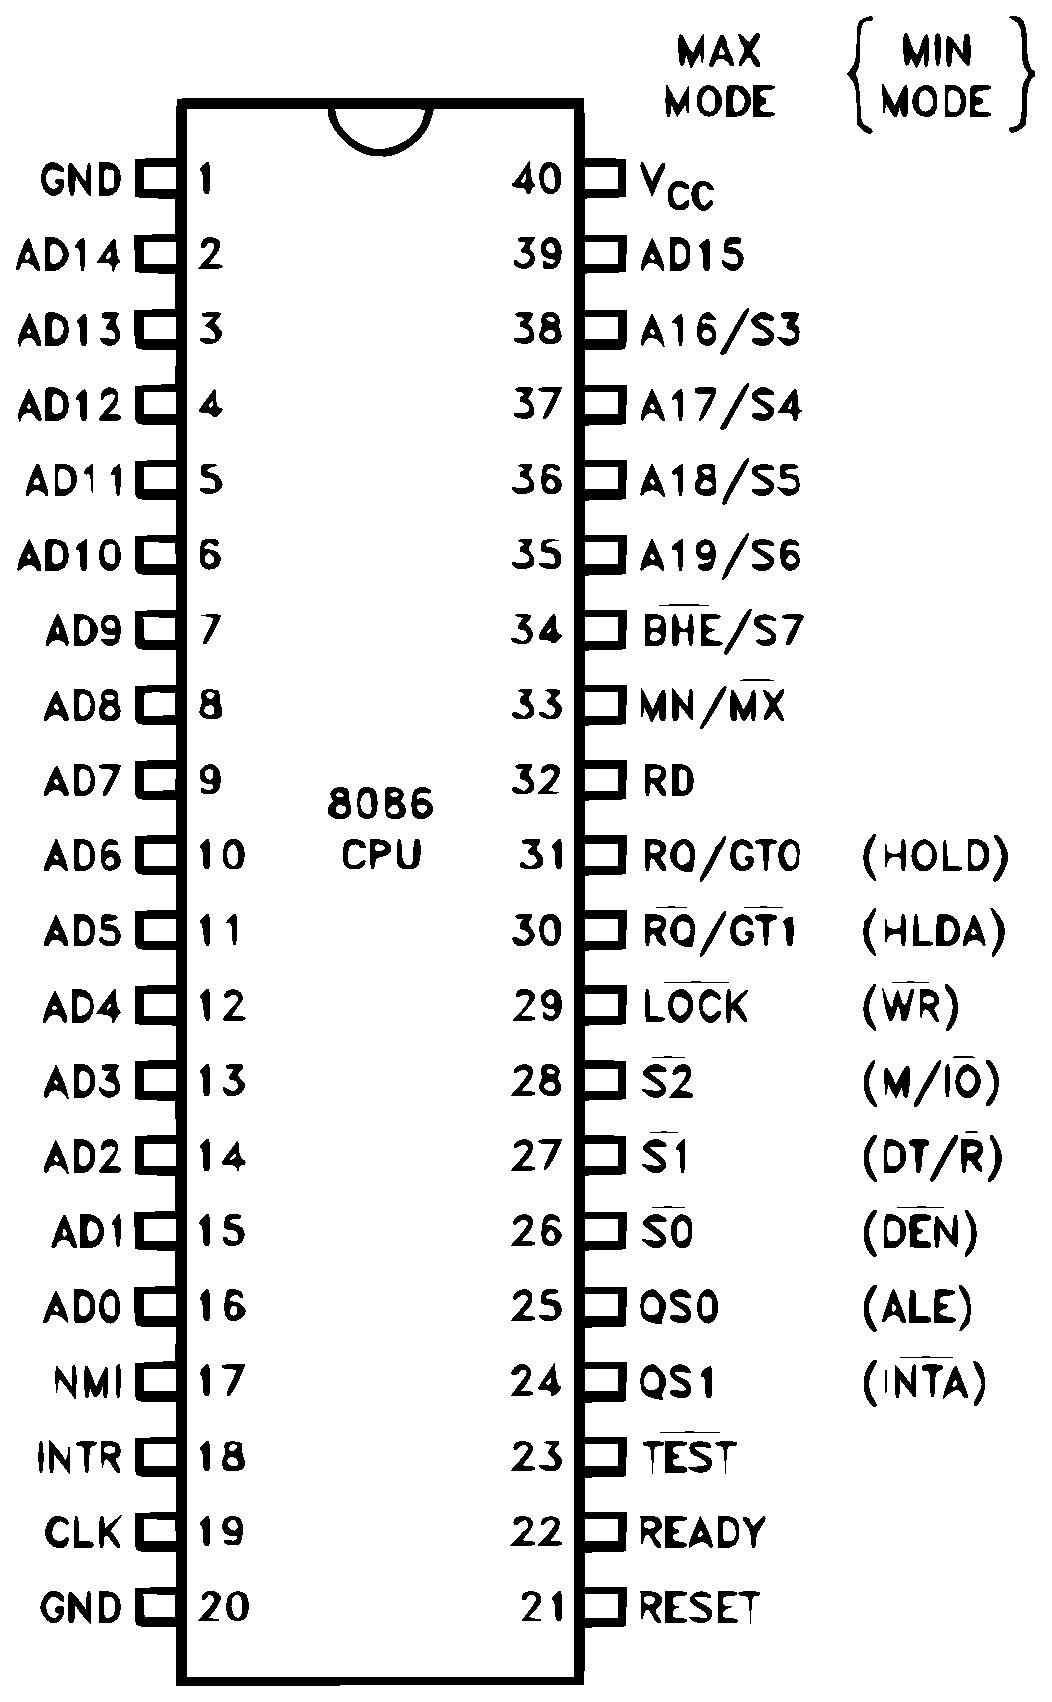
\includegraphics[scale=0.25]{figures/8086pinconfig.eps}
\caption{Pin configuration of the 8086 \cite{intel19908086}}
\label{fig:8086pinconfig}
\end{figure}
The processor has a multiplexed 20-bit address bus and 16-bit data bus: 16 pins are shared between both the address and data bus. The remaining higher order 4 bits in the address bus come from physical address calculation by the bus interface unit (BIU).\\
The processor can be operated along with other processors by putting it in maximum mode. This is done by strapping its MN/$\overline{\text{MX}}$ pin to the ground. In this mode, CPU encodes its signal, which are decoded and used by the 8288 bus controller to control the system. To put the processor in minimum mode, MN/$\overline{\text{MX}}$ pin is strapped to +5V.

\subsubsection{Execution Unit and Bus Interface Unit}
In section 2.3.3 and 2.3.4 we discussed how the efficiency of computation by mainframes was maximized by using batch system and multiprogramming. The idea was to minimize the time for which the processor was idle by giving it enough jobs/programs to keep it occupied while the I/O operations were performed by cheaper machines. The concept of batch system and multiprogramming were applied in the design of the 8086 microprocessor. Instead of having a single processing unit which was responsible for fetch and writing data and instructions and execution, the 8086 has two processing units: the execution unit (EU) and the bus interface unit (BIU). The EU is responsible for executing the instructions and the BIU is responsible for fetching instructions, reading operands, and writing data to memory or to the ports. The two processors operate independently of each other thus ensuring that the EU is in operation for most of the time. The BIU has an internal buffer in which it would prefetch and store the instructions so that the EU's time is not wasted by waiting for the next instruction. This buffer is basically a queue. The size of this queue is four bytes for the 8088 and six bytes for the 8086 \cite{intel19908086}.
\begin{figure}[h]
  \centering
  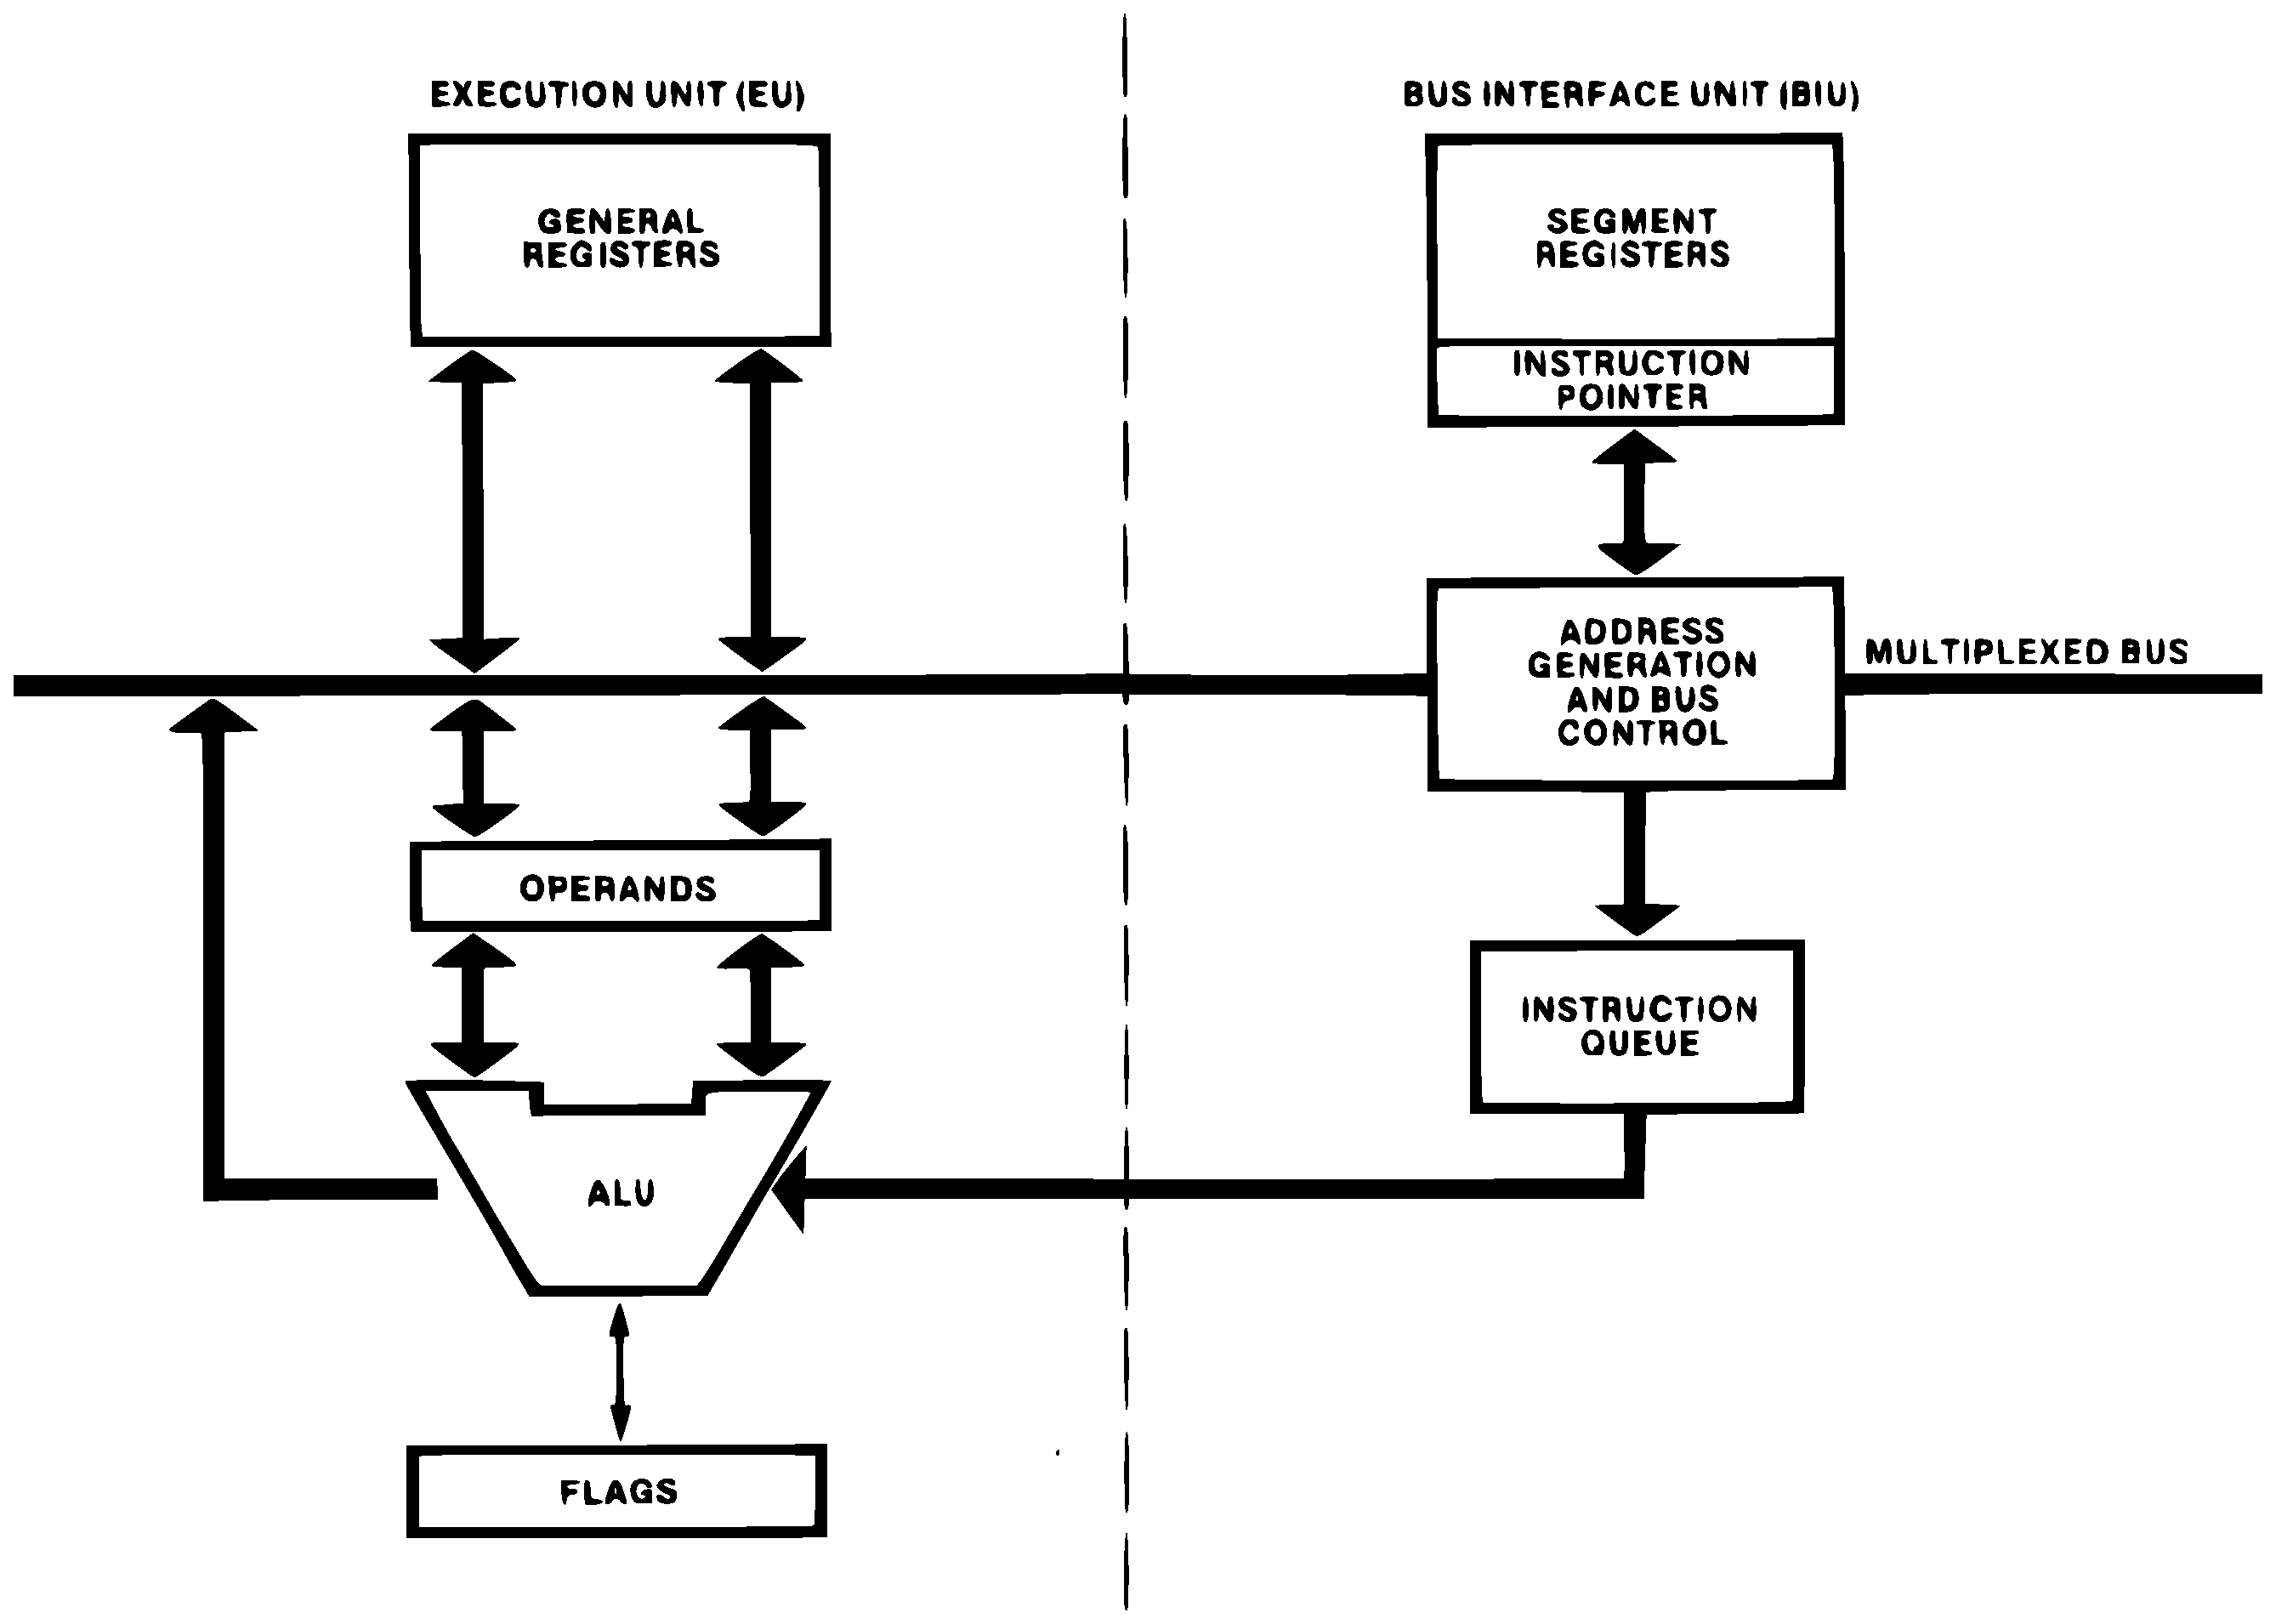
\includegraphics[scale=0.25]{figures/8086block.eps}
  \caption{Block diagram of the 8086/8088 microprocessor \cite{intel1979the}}
\label{fig:8086block}
\end{figure}

\subsubsection{Registers}
Two sets of registers are provided to both the EU and the BIU. The 16-bit registers provided to the EU are called general purpose registers. The 16-bit registers provided to the BIU are called segment registers. A 16-bit instruction pointer is also provided to the BIU.\\
General purpose registers are frequently used in arithmetic and logical calculations, and comparisons, and also for addressing data in memory. These are \verb|ax|, \verb|bx|, \verb|cx|, \verb|dx|, \verb|sp|, \verb|bp|, \verb|si|, and \verb|di|\footnote[1]{In older documents and source codes, one would find that instructions, operands, and hexadecimal numbers were exclusively written in uppercase. Nowadays, assembly source codes are written both in lowercase and uppercase literals. Due to the availability of different typesetting software, many newer documents also make use of both the cases for instructions, operands, and hexadecimal numbers. In this report and the source code for this project, instructions, register names, and hexadecimal numbers are exclusively written in lowercase. A breaks in this convention might be observed, especially at places where older documents are referenced, and in figures. In the end, the case which appears to be pleasant to the eyes and is relevant is used.}. Each of \verb|ax|, \verb|bx|, \verb|cx|, and \verb|dx| could be split into two 8-bit registers thus providing a total eight 8-bit registers. This is shown in \autoref{fig:8086gpr}. \verb|ax|, \verb|bx|, \verb|cx|, and \verb|dx| are used in computations and comparisons. One can say that there are four 16-bit accumulators in the 8086 processor. The \verb|ax| register along with \verb|dx| is used to store the results of operations. After 16-bit multiplication, the product's low word is stored in \verb|ax| and high word is stored \verb|dx|. After 16-bit division, the quotient is stored in \verb|ax| and the remainder in \verb|dx|. \verb|cx| register is used as a counter in loop operations.\\
\begin{figure}[h]
\centering
  \begin{subfigure}{.5\textwidth}
  \centering
  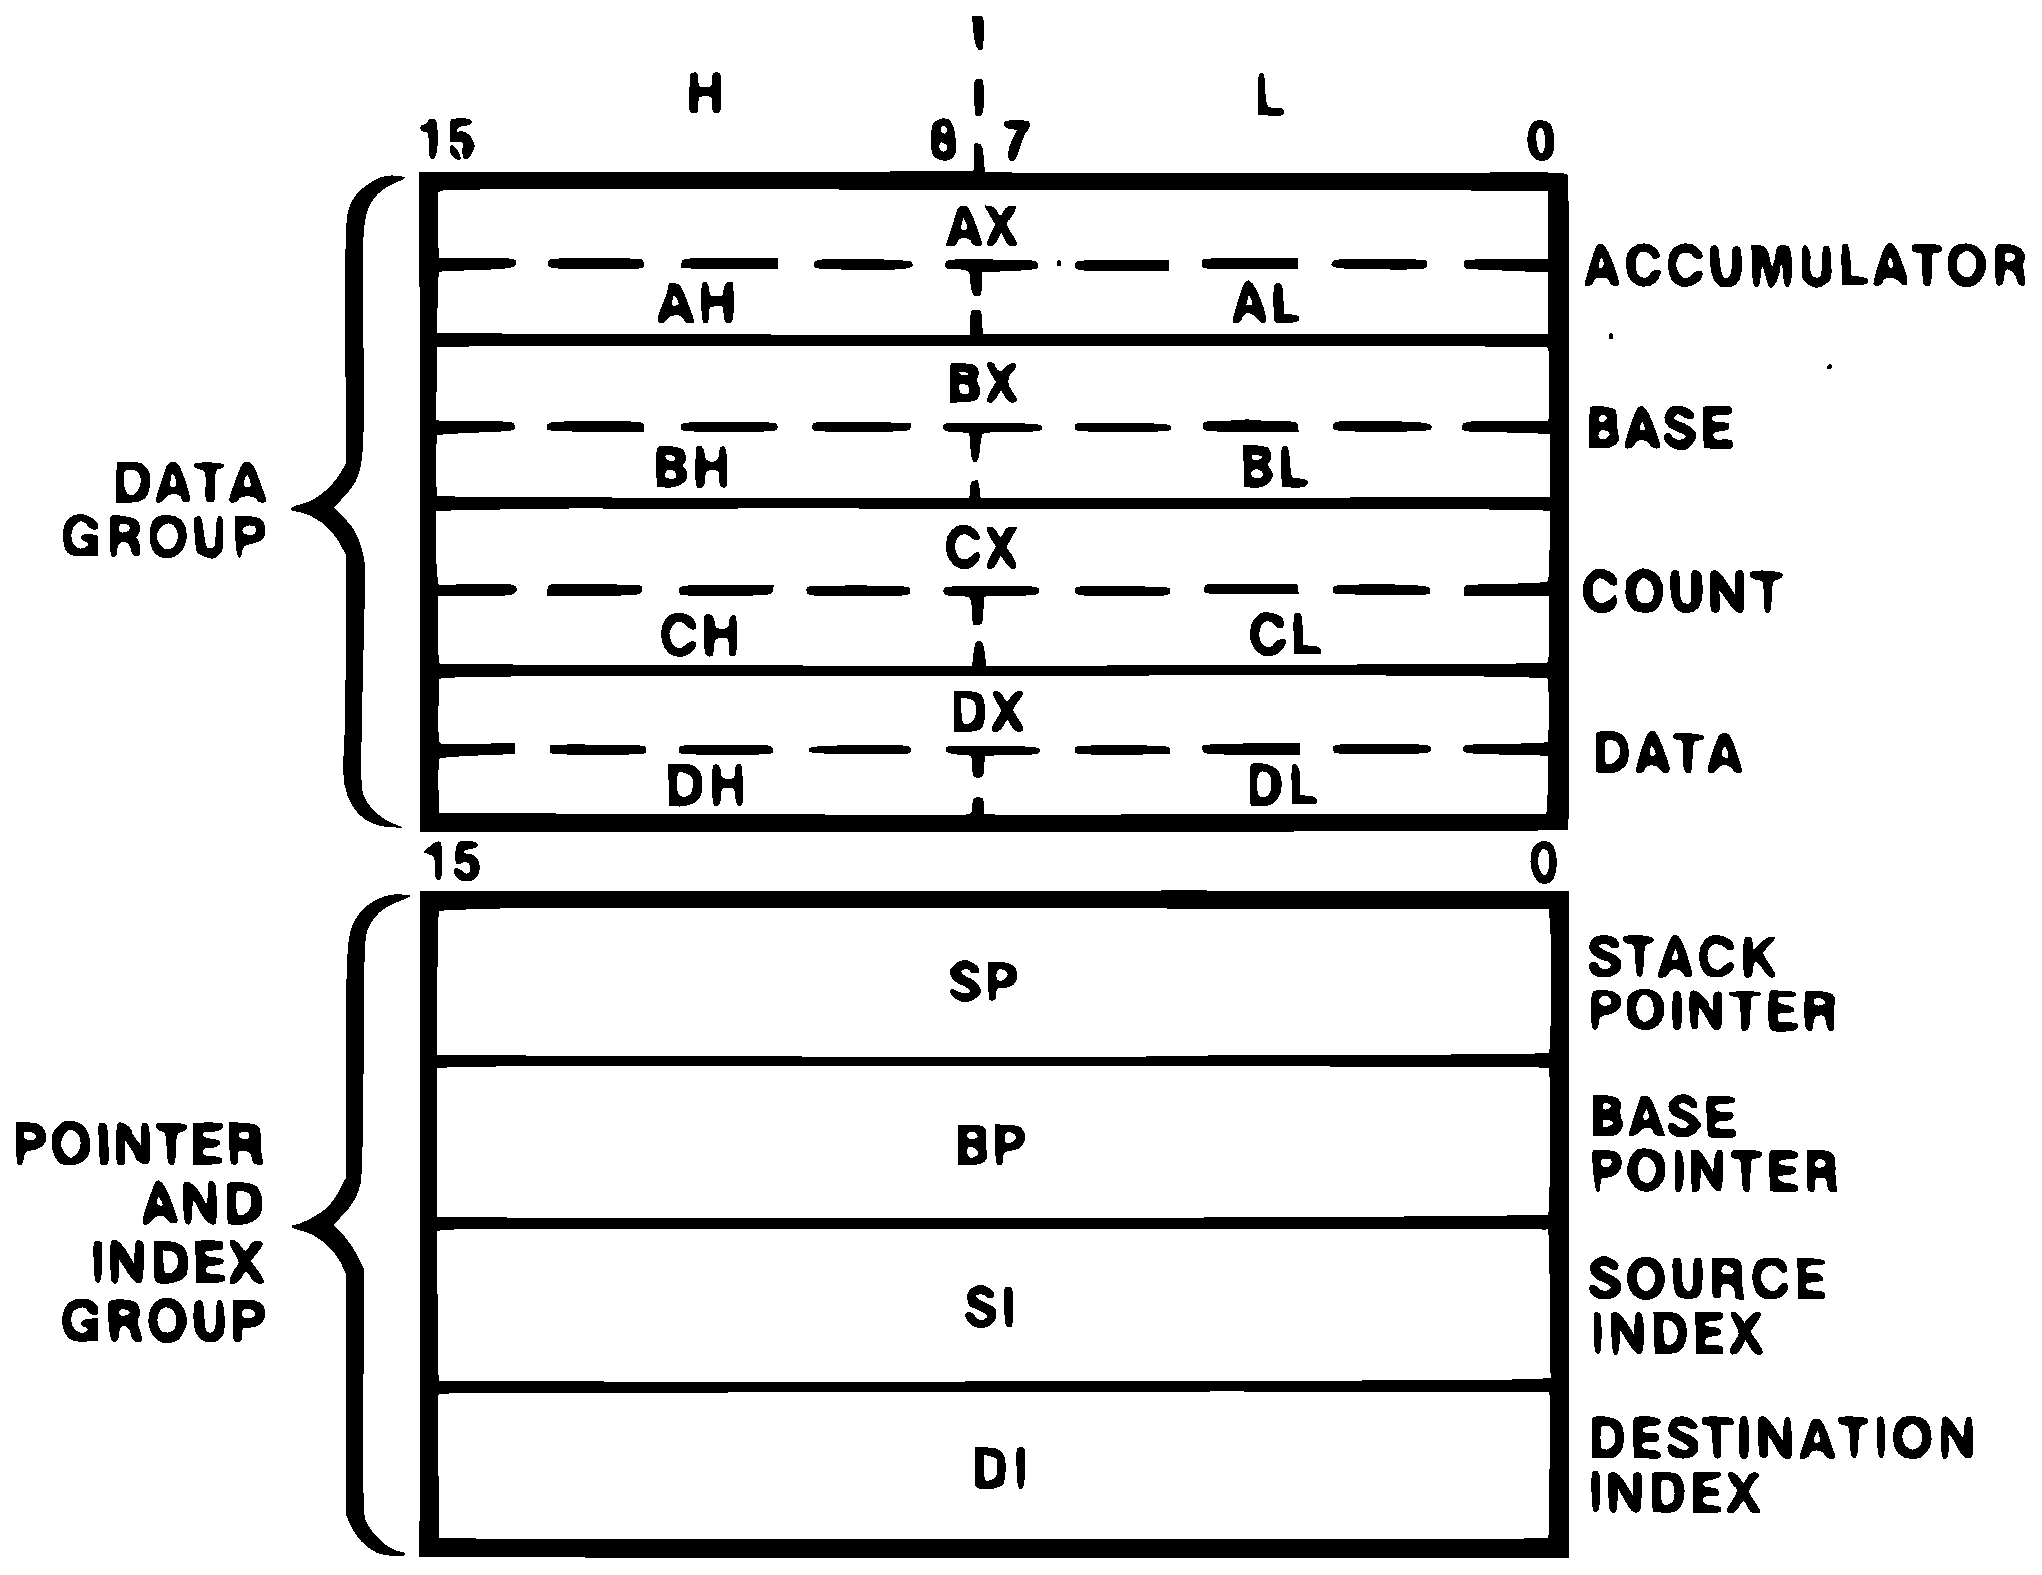
\includegraphics[scale=0.25]{figures/8086gpr.eps}
  \caption{General purpose registers}
  \label{fig:8086gpr}
  \end{subfigure}%
  \begin{subfigure}{.5\textwidth}
  \centering
  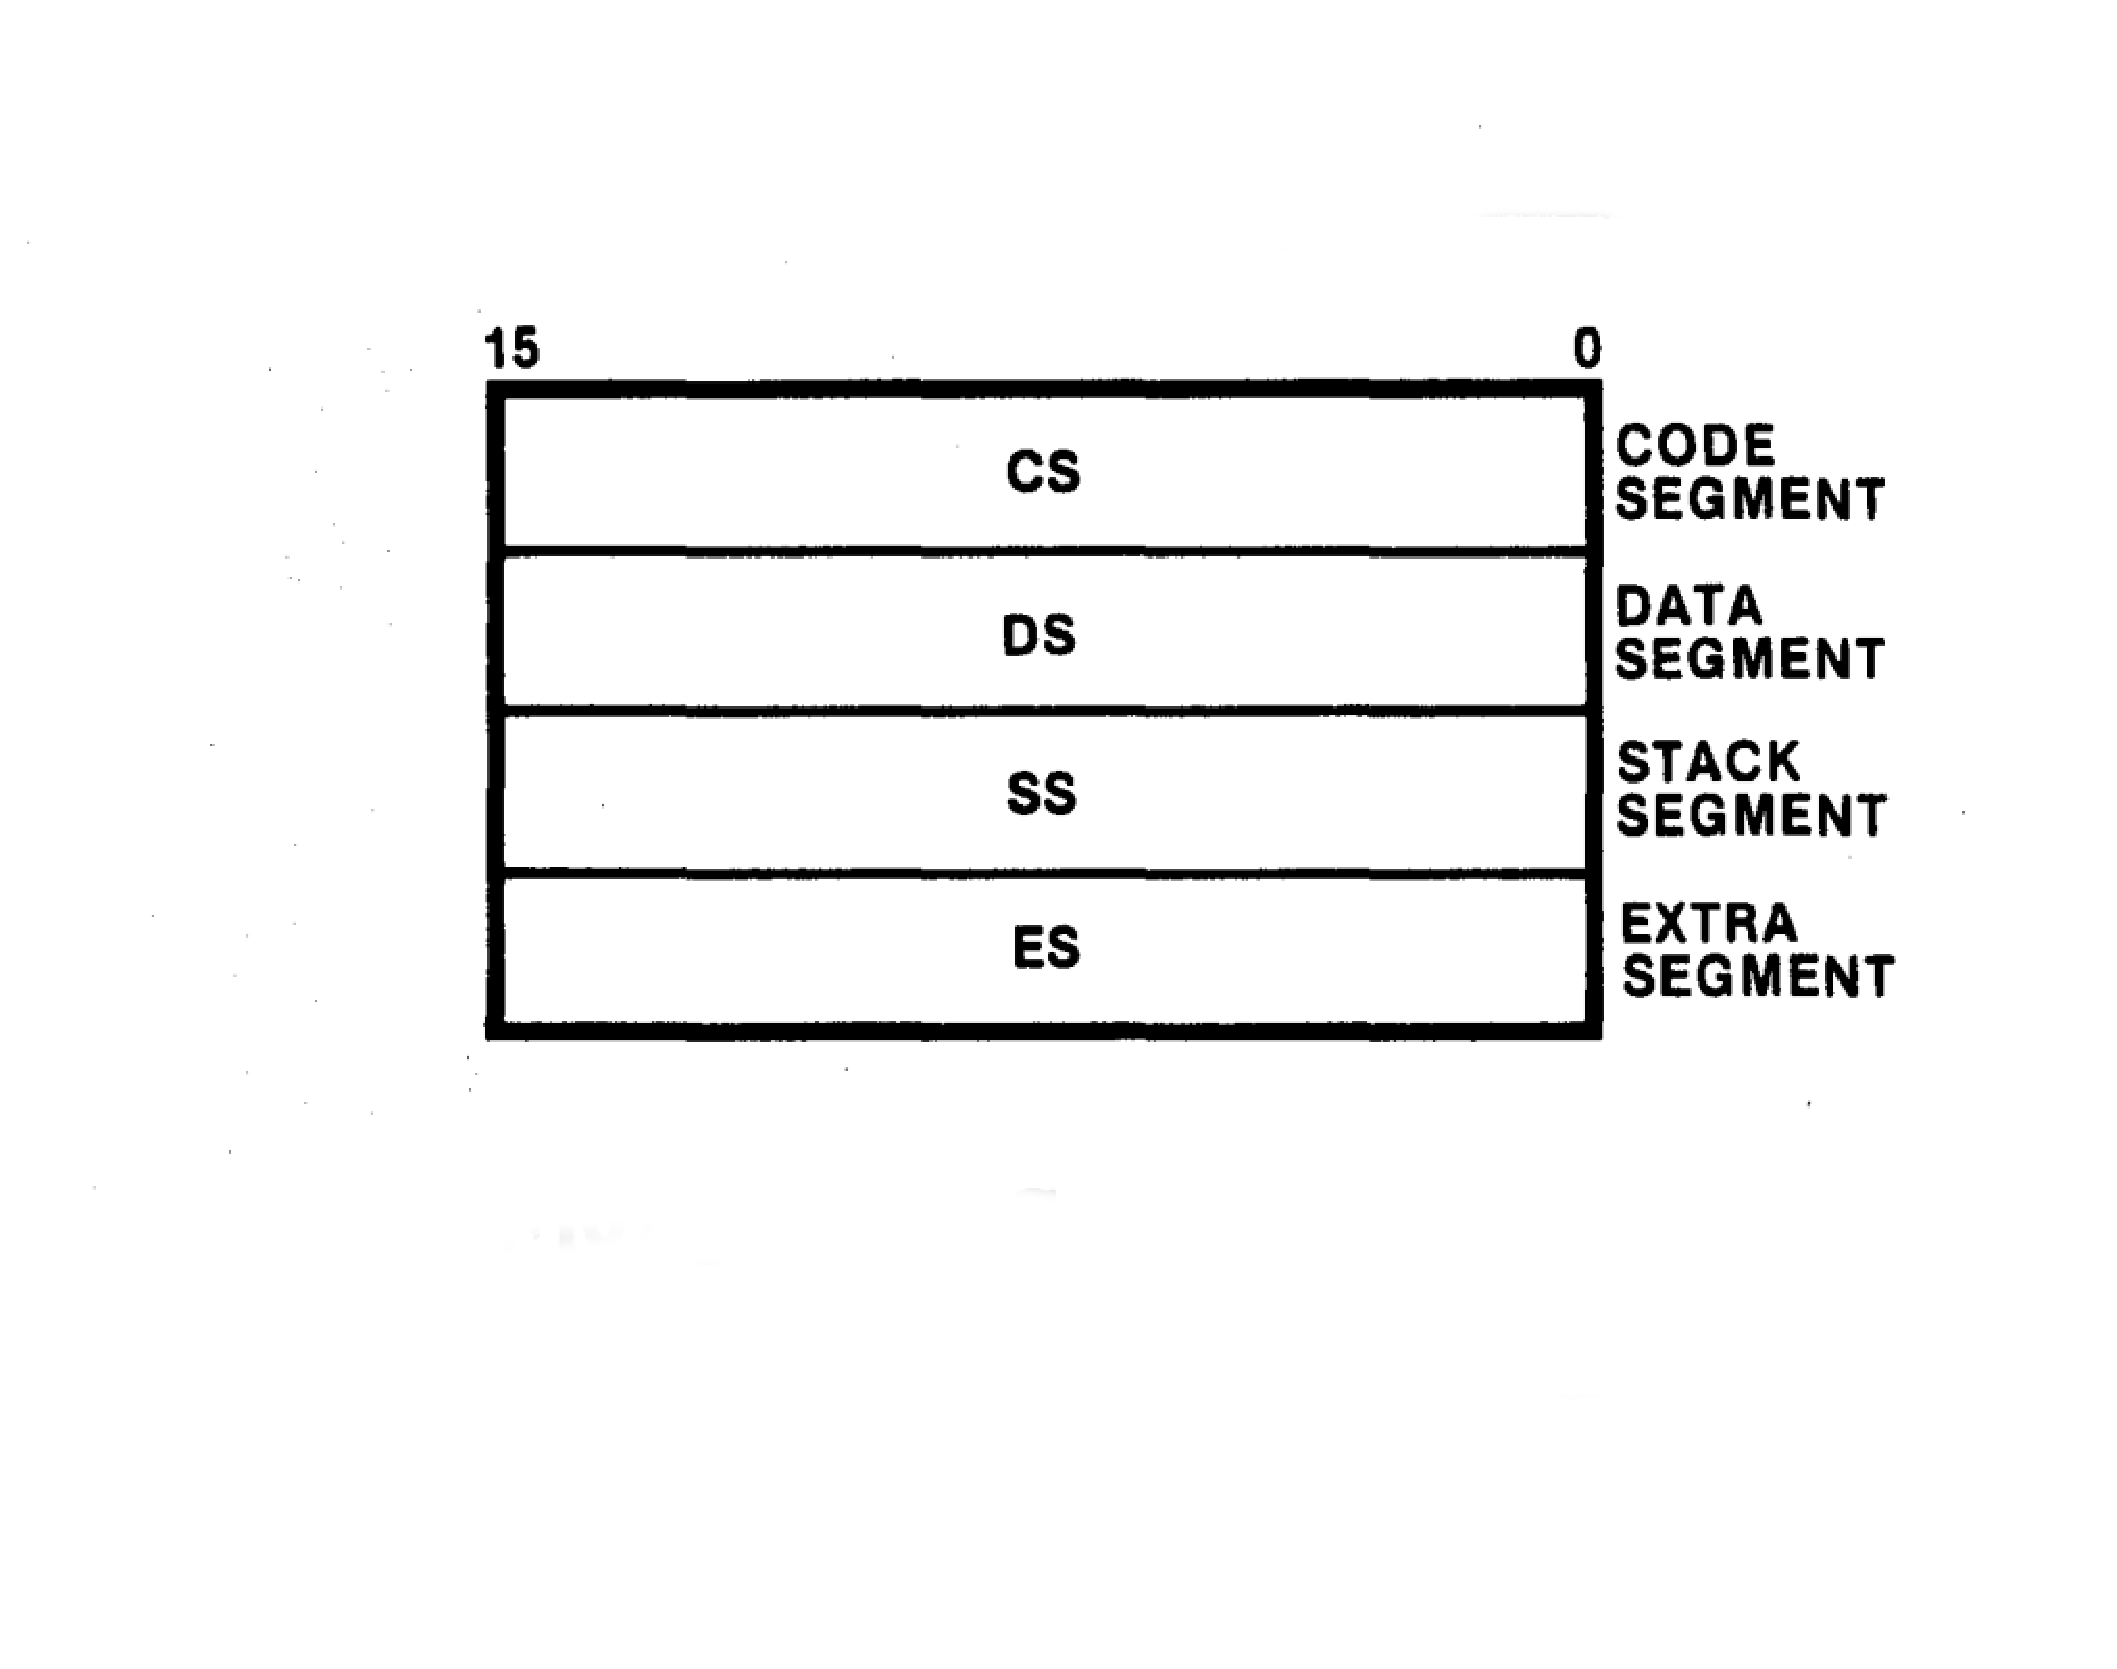
\includegraphics[scale=0.25]{figures/8086segr.eps}
  \caption{Segment registers}
  \label{fig:8086segr}
  \end{subfigure}
  \newline
  \begin{subfigure}{0.9\textwidth}
  \centering
  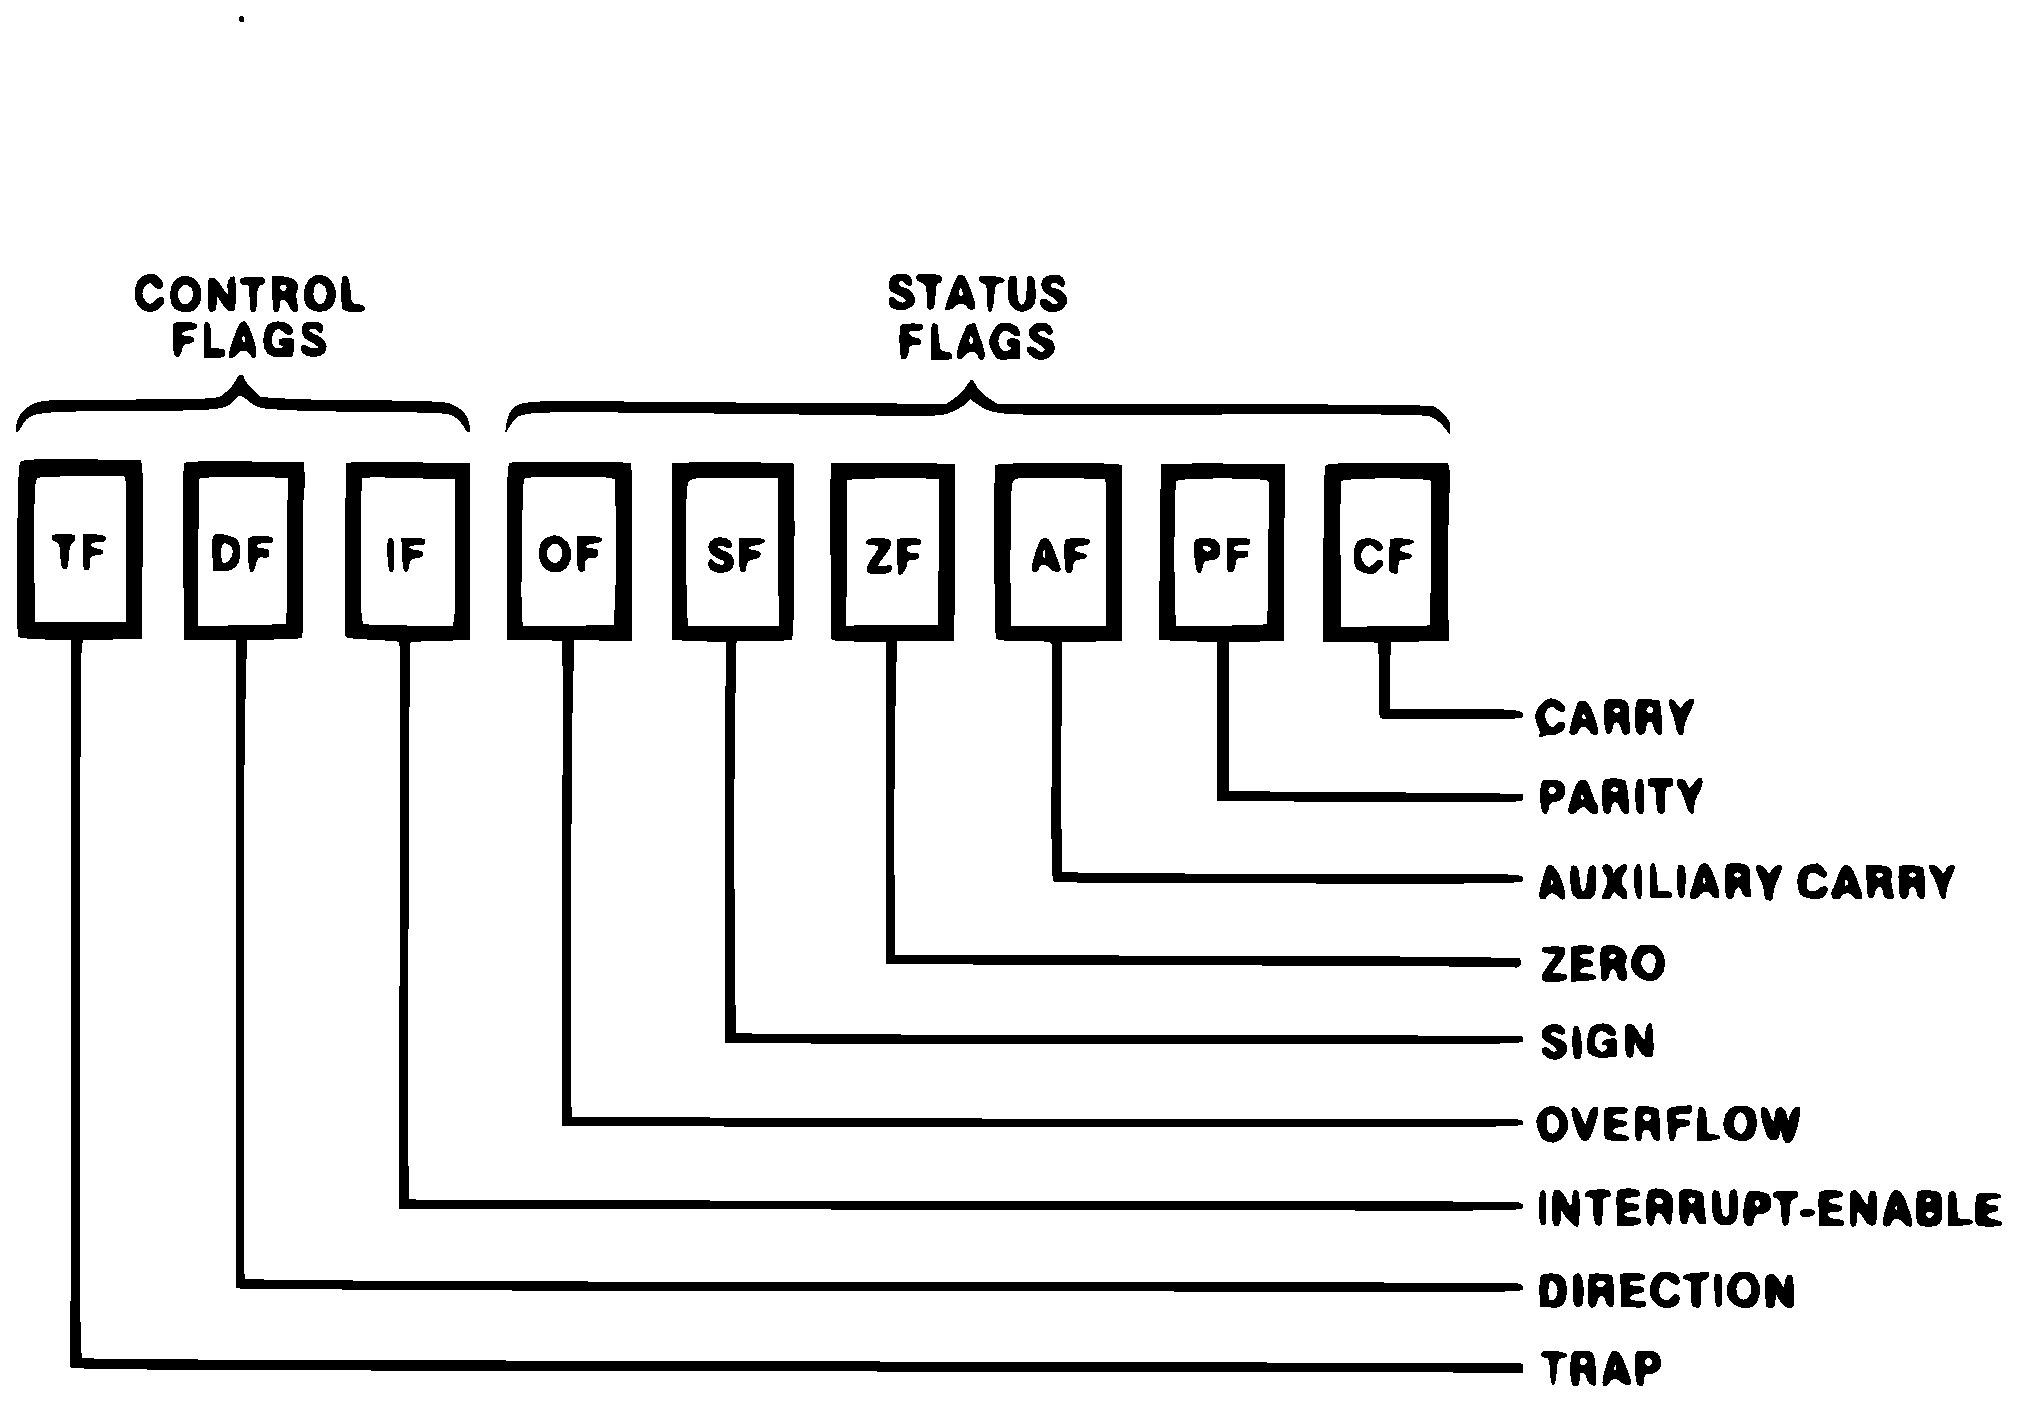
\includegraphics[scale=0.25]{figures/8086flags.eps}
  \caption{Flags}
  \label{fig:8086flag}
  \end{subfigure}
 \caption{8086 registers \cite{intel1979the}}
\end{figure}
The stack pointer register, \verb|sp|, and the base pointer register, \verb|bp|, are used for setting up stack frames and for accessing parameters passed to the functions. The source index register, \verb|si|, and the destination index register, \verb|di|, are used to provide the index of a single byte (or word) of source and destination strings, respectively.\\
\verb|bx| and \verb|bp| are used to provide the base address of a data structure or the stack frame. \verb|si| and \verb|di| are used to index through these data structures.\\
Segment registers are the "hack" which allow programmers to access 1 MiB of memory instead of mere 64 kiB. There are four 16-bit segment registers which are available to the BIU: code segment (\verb|cs|), data segment (\verb|ds|), extra segment (\verb|es|), and stack segment (\verb|ss|) registers (\autoref{fig:8086segr}). The purpose of segment registers is now presented.\\
A 16-bit register can address only 64 kiB of memory, with addresses of bytes going from 0x0000 to 0xffff (0 - 65535). If a 16-bit base value is left shifted by 4 bits and added to another 16-bit number, the resulting sum is a 20-bit number which can have any value in the range 0x00000 - 0xfffff (0 - 1048575). A 20-bit variable can address 1 MiB of memory. This is exactly how \textit{physical addresses} are generated from \textit{effective addresses}. In 8086, memory is divided in chunks, with the maximum size of chunks being 64 kiB. These chunks are called segments. The address at which a chunk starts is called segment base address. Segment base addresses are right-shifted by 4 bits and stored in segment registers. The effective address of a data or instruction byte is the offset at which that byte is located from the segment base address. Effective addresses can be stored in a general purpose register (in the case of data) or in the 16-bit instruction pointer, \verb|ip| (in the case of an instruction). To access the given data/instruction in a block, the BIU left-shifts the value stored in the segment register by 4 bits and to it adds the 16-bit effective address. The resulting 20-bit number is the physical address of the required data or instruction byte. The following relations will clarify the process of physical address generation.
\begin{enumerate}
  \item physical address of an instruction = (\verb|cs| $<<$ 4) + \verb|ip|
  \item \begin{enumerate}
    \item[a.] Byte or word in source string = (\texttt{ds} $<<$ 4) + \texttt{si}
    \item[b.] Byte or word in destination string =  (\texttt{es} $<<$ 4) + \texttt{di}
  \end{enumerate}
  \item physical address of a data byte = (\verb|ds|/\verb|es| $<<$ 4) + base address (\verb|bx|/\verb|bp|)\\
  \hspace*{8.7cm} + index (\verb|si|/\verb|di|)\\ 
  \hspace*{8.7cm} + diplacement (8-bit or 16-bit)
  \item address of the base of a stack frame = (\verb|ss| $<<$ 4) + \verb|bp|
  \item address of the top of a stack frame = (\verb|ss| $<<$ 4) + \verb|sp|
\end{enumerate}
As the value of lower nibble of the 20-bit segment base address is always zero, therefore, two segments have at least a gap of 16 bytes between them.\\
Besides the general purpose registers, the EU is also provided with a flag register having status and control flags (\autoref{fig:8086flag}). Status flags contain the represent the state of the machine after last operation (overflow, parity, carry bits, etc.). Control flag alter the way programs are executed by (direction of increment of index registers, interrupts, and single-step mode).

\subsubsection{Endianness}
The order in which a processor stores the high byte and low byte of a word is called \textit{endianness}. There are two types of endianness: little endianness and big endianness. If a processor stores the least significant byte at a lower address and most significant byte at higher address, then it is said to follow little-endian byte ordering. if a processor stores the most significant byte at a lower address and least significant byte at higher address, then it is said to be using big-endian byte ordering. 8086 follows little-endian byte-ordering. It should be noted that little-endian ordering is not applicable for values stored in registers. Therefore, if register \verb|ax| stores the number 0x1234, then \verb|al| will be storing 0x34 and \verb|ah| will be storing 0x12. On the other hand, if a memory location, say 0x1000 is said to store 0x1234, then 0x34 will stored at the address 0x1000, and 0x12 will be stored at the address 0x1001 (\autoref{fig:littlendian}).
\begin{figure}[h]
  \centering
  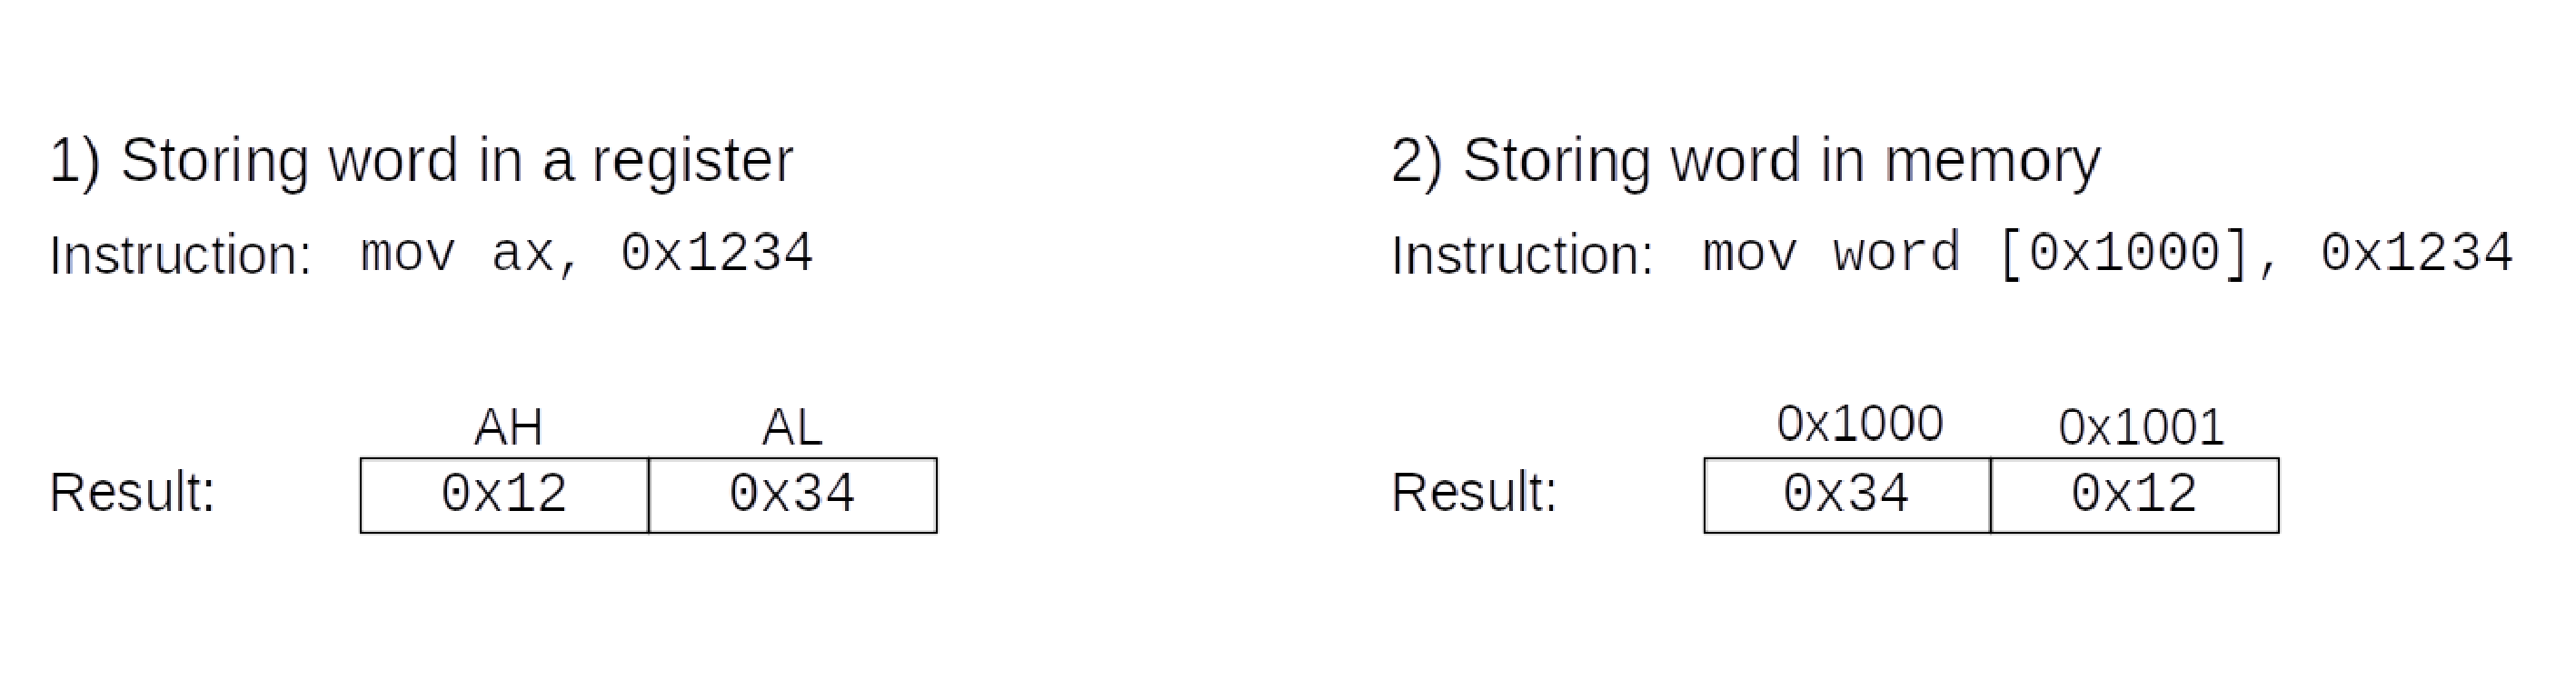
\includegraphics[scale=0.25]{figures/wordendian.eps}
  \caption{Ordering of bytes of words in registers and memory}
\label{fig:littlendian}
\end{figure}
Another type of data variable is a doubleword. A doubleword, as the name suggests, consists of two words and is used to store memory addresses. Therefore, it is often called as a pointer. As has already been discussed in section 2.4.3, physical address is made up of segment base address and an offset value. A doubleword's most significant word contains the segment base address, and its least significant word contains the offset of the data/instruction to be accessed. A doubleword is stored in memory by storing the least significant word (which contains the offset) at the lower address, and then storing the most significant word (which contains the segment base address) (\autoref{fig:doublewords}).
\begin{figure}[h]
  \centering
  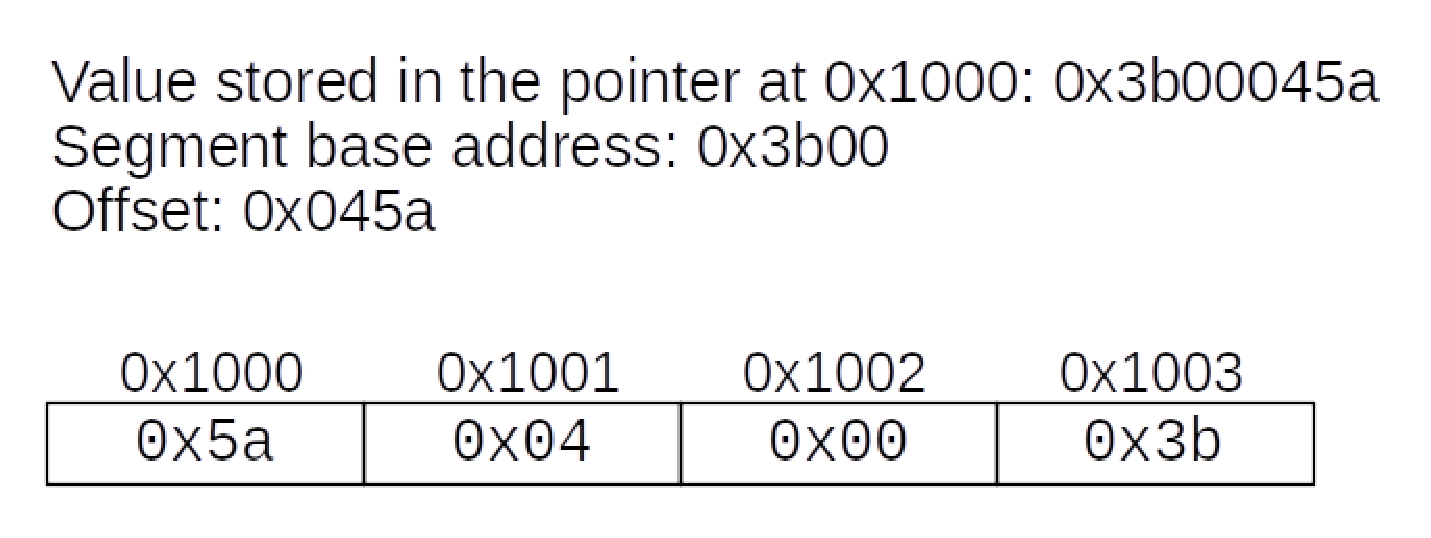
\includegraphics[scale=0.25]{figures/doublewords.eps}
  \caption{Storing doublewords in memory}
\label{fig:doublewords}
\end{figure}
This storing convention is most often used in intersegment calls where the calle's segment base address are first pushed onto the stack and the offset is pushed afterwards. After this, the far call instruction is executed, which pushes the current \verb|cs|'s and then \verb|ip|'s value onto the stack This is shown in \autoref{fig:stackops}. From the figure note that the stack grows downwards towards the base address of the segment in which the stack is kept.
\begin{figure}[h]
  \centering
  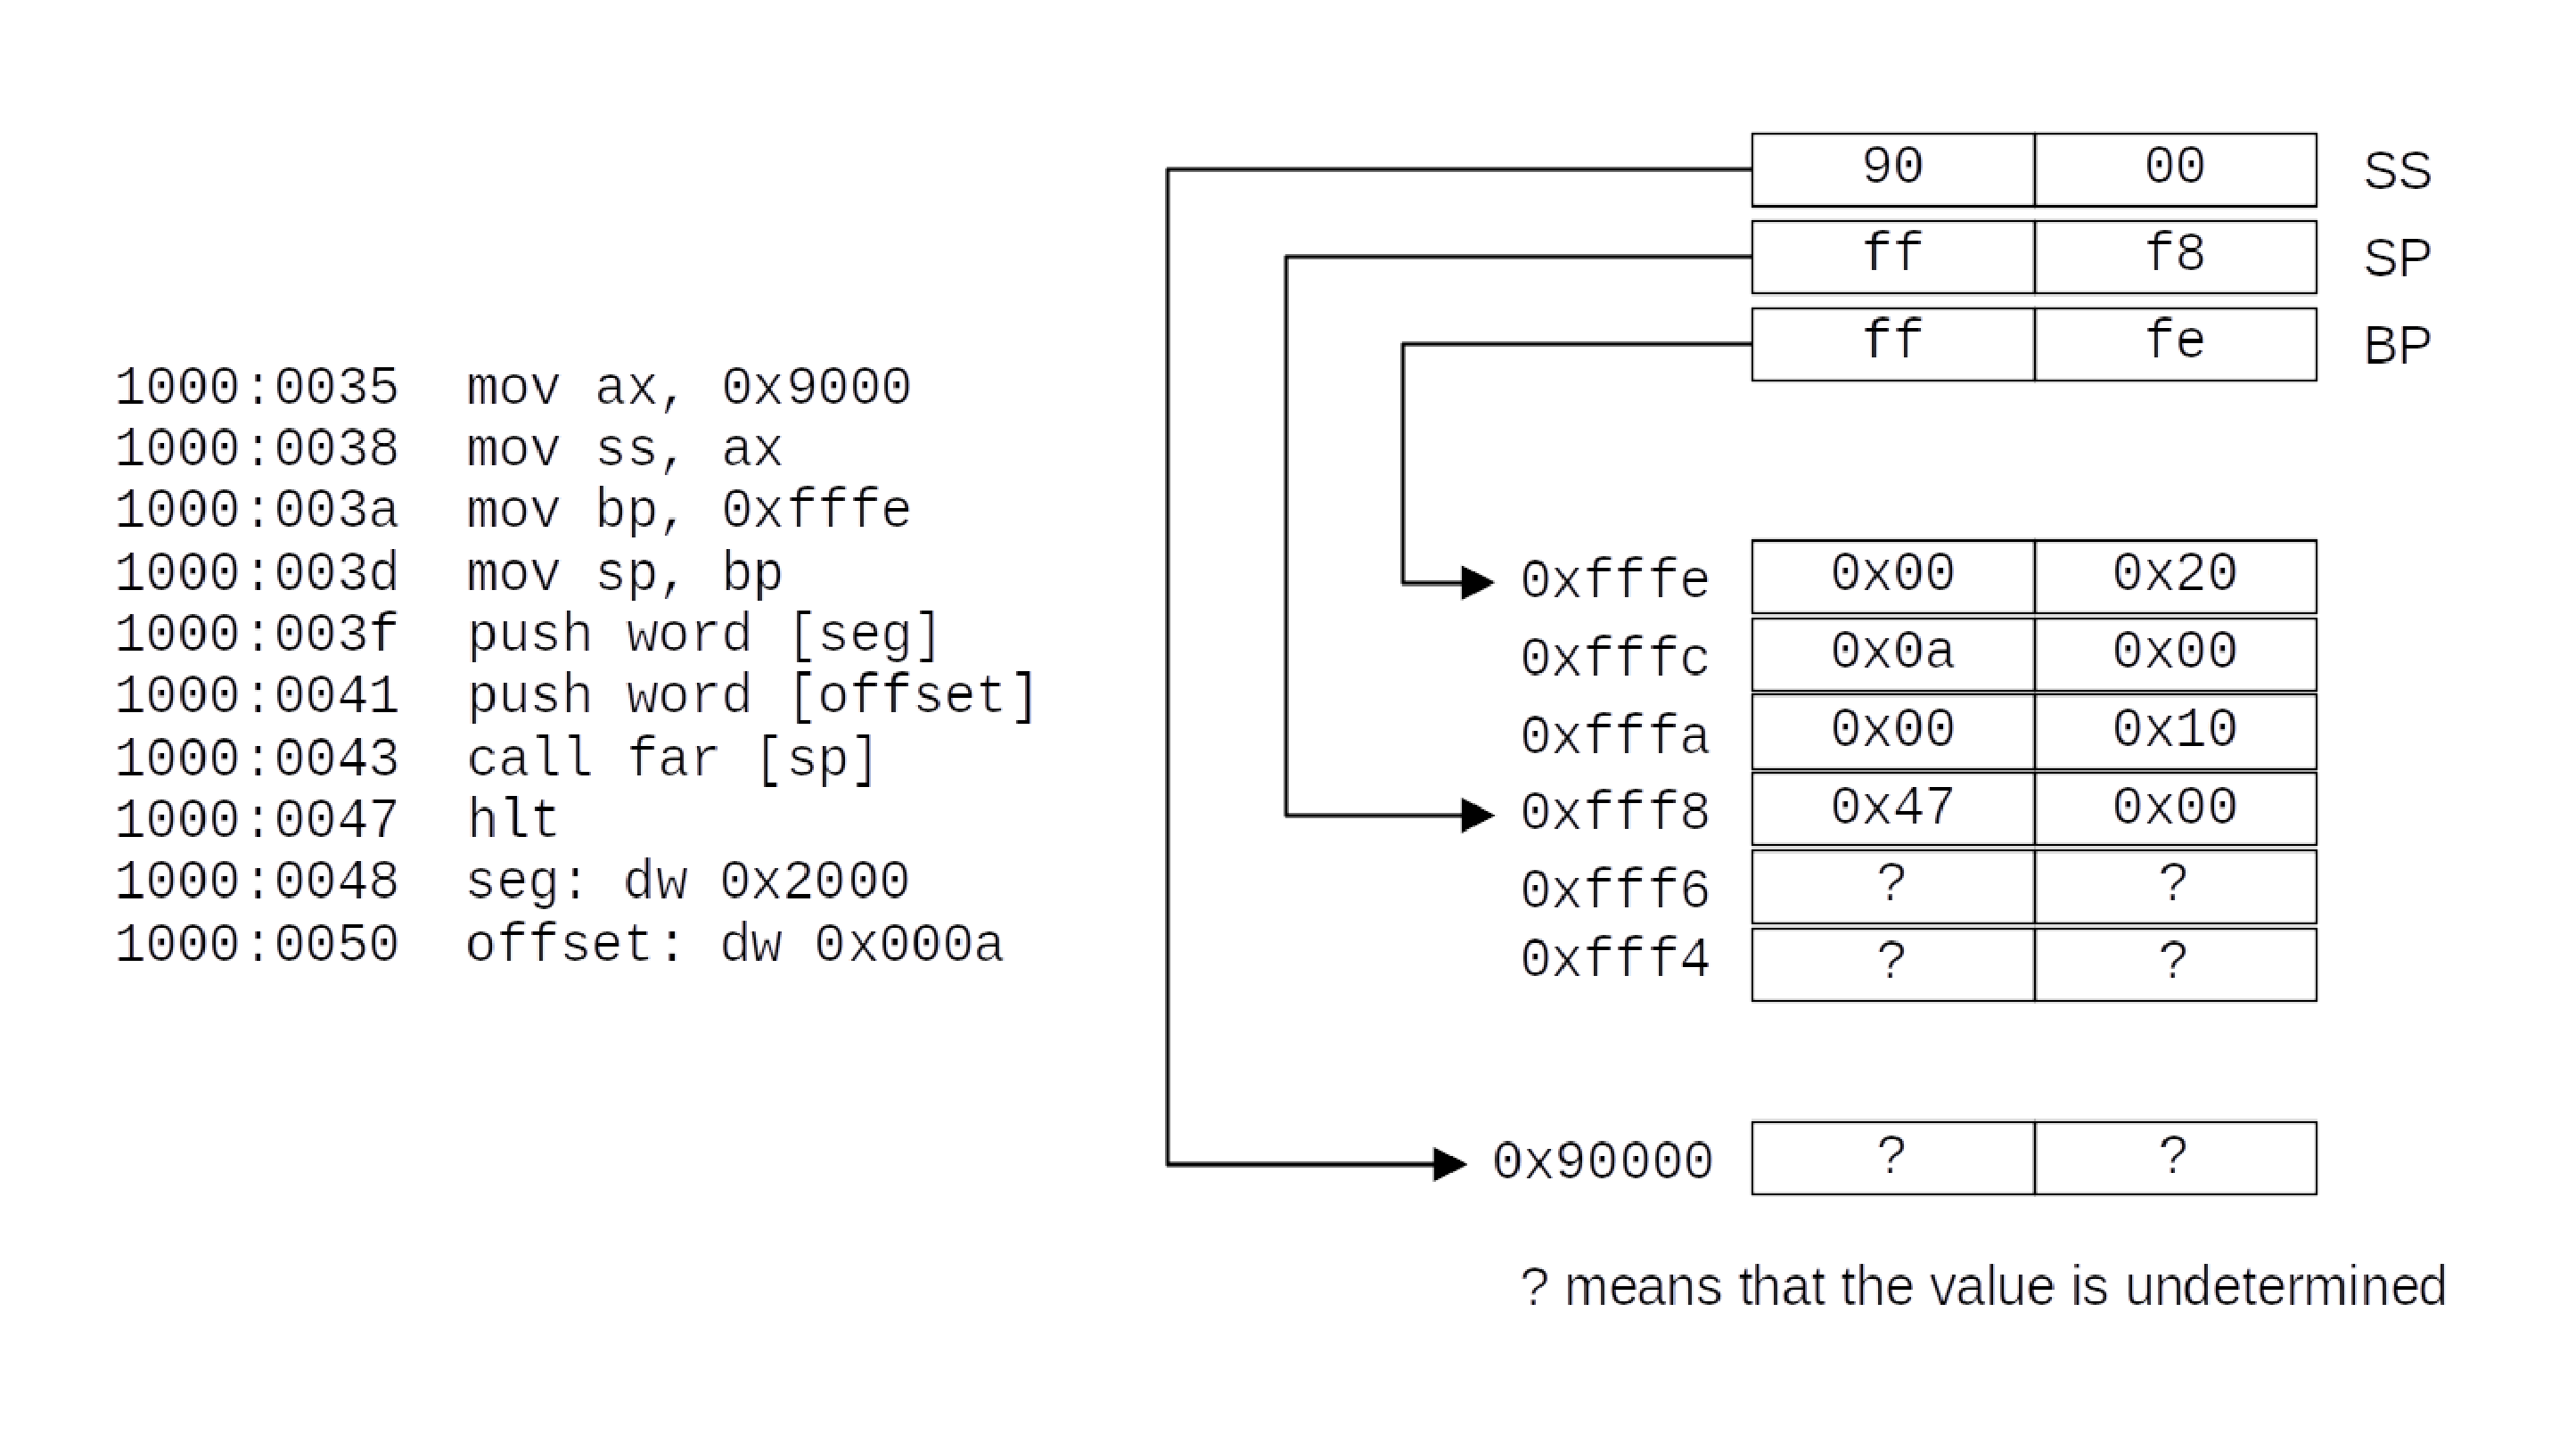
\includegraphics[scale=0.25]{figures/stackop.eps}
  \caption{Storing pointers on stack during intersegment calls}
\label{fig:stackops}
\end{figure}

\subsubsection{Addressing Modes}
Programming in 8086 assembly language is easier and enjoyable in comparison to programming in 8085's (or earlier microprocessor's) assembly language. This is because of the availability of powerful arithmetic, loop and string instructions, as well as the presence of different types of addressing modes. The addressing modes of 8086 are given below:
\begin{enumerate}
  \item \textit{Immediate Addressing}: Operand is provided in the instruction itself.\\Example: \verb|mov ax, 0x1234|.
  \item \textit{Register Addressing}: Both the operands are registers. Example: \verb|xor cx, cx|.
  \item \textit{Direct Addressing}: Effective address is provided in the instruction itself.\\Example: \verb|add ax, word [var1]|.
  \item \textit{Register Indirect Addressing}: The effective address is stored in base registers (\verb|bx| and \verb|bp|) or index registers (\verb|si| and \verb|di|). Example: \verb|mov al, byte [si]|. 
  \item \textit{Based Addressing}: The effective address used in the instruction is the sum of the value stored in a base register and a displacement. Using \verb|bp| as the base register allows us to access parameters of a function. Using \verb|bx| as the base register allows us to access data in a structure. Example: \verb|mov ax, word [bp + 2]|.
  \item \textit{Indexed Addressing}: Effective address is calculated from the sum of displacement and the value stored in one of the index registers. This is useful for accessing elements of an array. Example: \verb|mov dl, byte [si]|.
  \item \textit{Based Indexed Addressing}: The effective address is computed by adding a displacement, the value stored in a base register, and an index register. This addressing mode is useful in accessing elements of a parameter which might be a data structure. Example: \verb|mov dl, byte [bp + si + 4]|.
  \item \textit{String Addressing}: String instructions involve the use of string registers (\verb|si| and \verb|di|) and instructions. When string instructions are executed, it is assumed that \verb|si| is a pointer to the first byte or word of the source string, and \verb|di| is a pointer to the first byte or word of the destination string. Either \verb|si|, or \verb|di|, or both are either incremented or decremented depending on whether the direction flag is cleared or set, respectively. Example: \verb|repne lodsb|.
  \item \textit{I/O Port Addressing}: Peripherals which have port addresses are accessed using \texttt{in} and \verb|out| instructions. In direct port addressing, the 8-bit port address is provided with the instruction itself. The value being read or written is contained in \verb|al|. In indirect port addressing, the 16-bit port address is present in the register \texttt{dx}. Example: \verb|out 0x70, al|.
\end{enumerate}

\subsection{Design of the original IBM PC}
The original IBM PC was released on August 12, 1981. Thanks to its cheaper price, easily available hardware and software, and marketing, the IBM PC standardised the personal computer market. Although IBM no longer manufactures PCs, the IBM PC and its successors are still the \textit{de facto} standard for PCs \cite{ibmarchpc}.

\subsubsection{Physical Specifications}
Due its lower price and IBM's familiarity with it, the original IBM PC contained the 8088 microprocessor with a clock rate of 4.77 MHz. Clones of the IBM PC were released less than an year later, and some of them, like the Amstrad PC1512, had the 8086 microprocessor.\\
Both 8088 and 8086 can access 1 MiB of memory. However, as this memory was fairly large and expensive in the early 1980s, most PCs came with 16 kiB to 640 kiB of memory. Expansion slots were often provided for the user to increase the memory of the system themselves.\\
The original IBM PC came with upto two 5.25'' 160 kiB floppy disk drives. A disk-drive adapter was provided to interface with the disk drives. Cassette tape recorder and hard disks were also supported. Later versions of the IBM PC came with hard disk drives.\\
Addressing of storage disks was done using cylinder-head-sector (CHS) addressing. A single disk or a platter, in general, has two readable sides. A pair of heads were used to read and write to the disk. A single side of the disk was divided into tracks. A single track is contained within two concentric hollow cylinders and is made up of sectors, with each sector having 512 bytes of memory (\autoref{fig:chs}). Numbering of sectors start from 1, but the numbering of cylinders and heads starts from zero. The equation given below gives us the total size of the disk.
\begin{center}
$M = M_s \times N_s \times N_t \times N_h$
\end{center}
where
\begin{center}\begin{tabular}{ccl}\
$M$ &= &total storage capacity of the disk\\
$M_s$ &= &storage capacity of a single sector\\
$N_s$ &= &total number of sectors per track\\
$N_t$ &= &total number of tracks per head\\
$N_h$ &= &total number of heads per disk\\ 
\end{tabular}\end{center}
Consider the case of a standard 3.5'' floppy disk. It has the following specifications:
\begin{center}\begin{tabular}{ccl}\
$M_s$ &= &512 bytes/sector\\
$N_s$ &= &18 sectors/track\\
$N_t$ &= &80 tracks/head\\
$N_h$ &= &2 heads/disk\\ 
\end{tabular}\end{center}
which gives us
\begin{center}\begin{tabular}{ccl}
$M$ &= &$512 \times 18 \times 80 \times 2$\\
 &= &1474560 bytes\\
 &= &1.44 MiB
\end{tabular}\end{center}
Modern operating systems frequently  use logical block addressing (LBA) instead of CHS.\\
\begin{figure}[h]
  \centering
  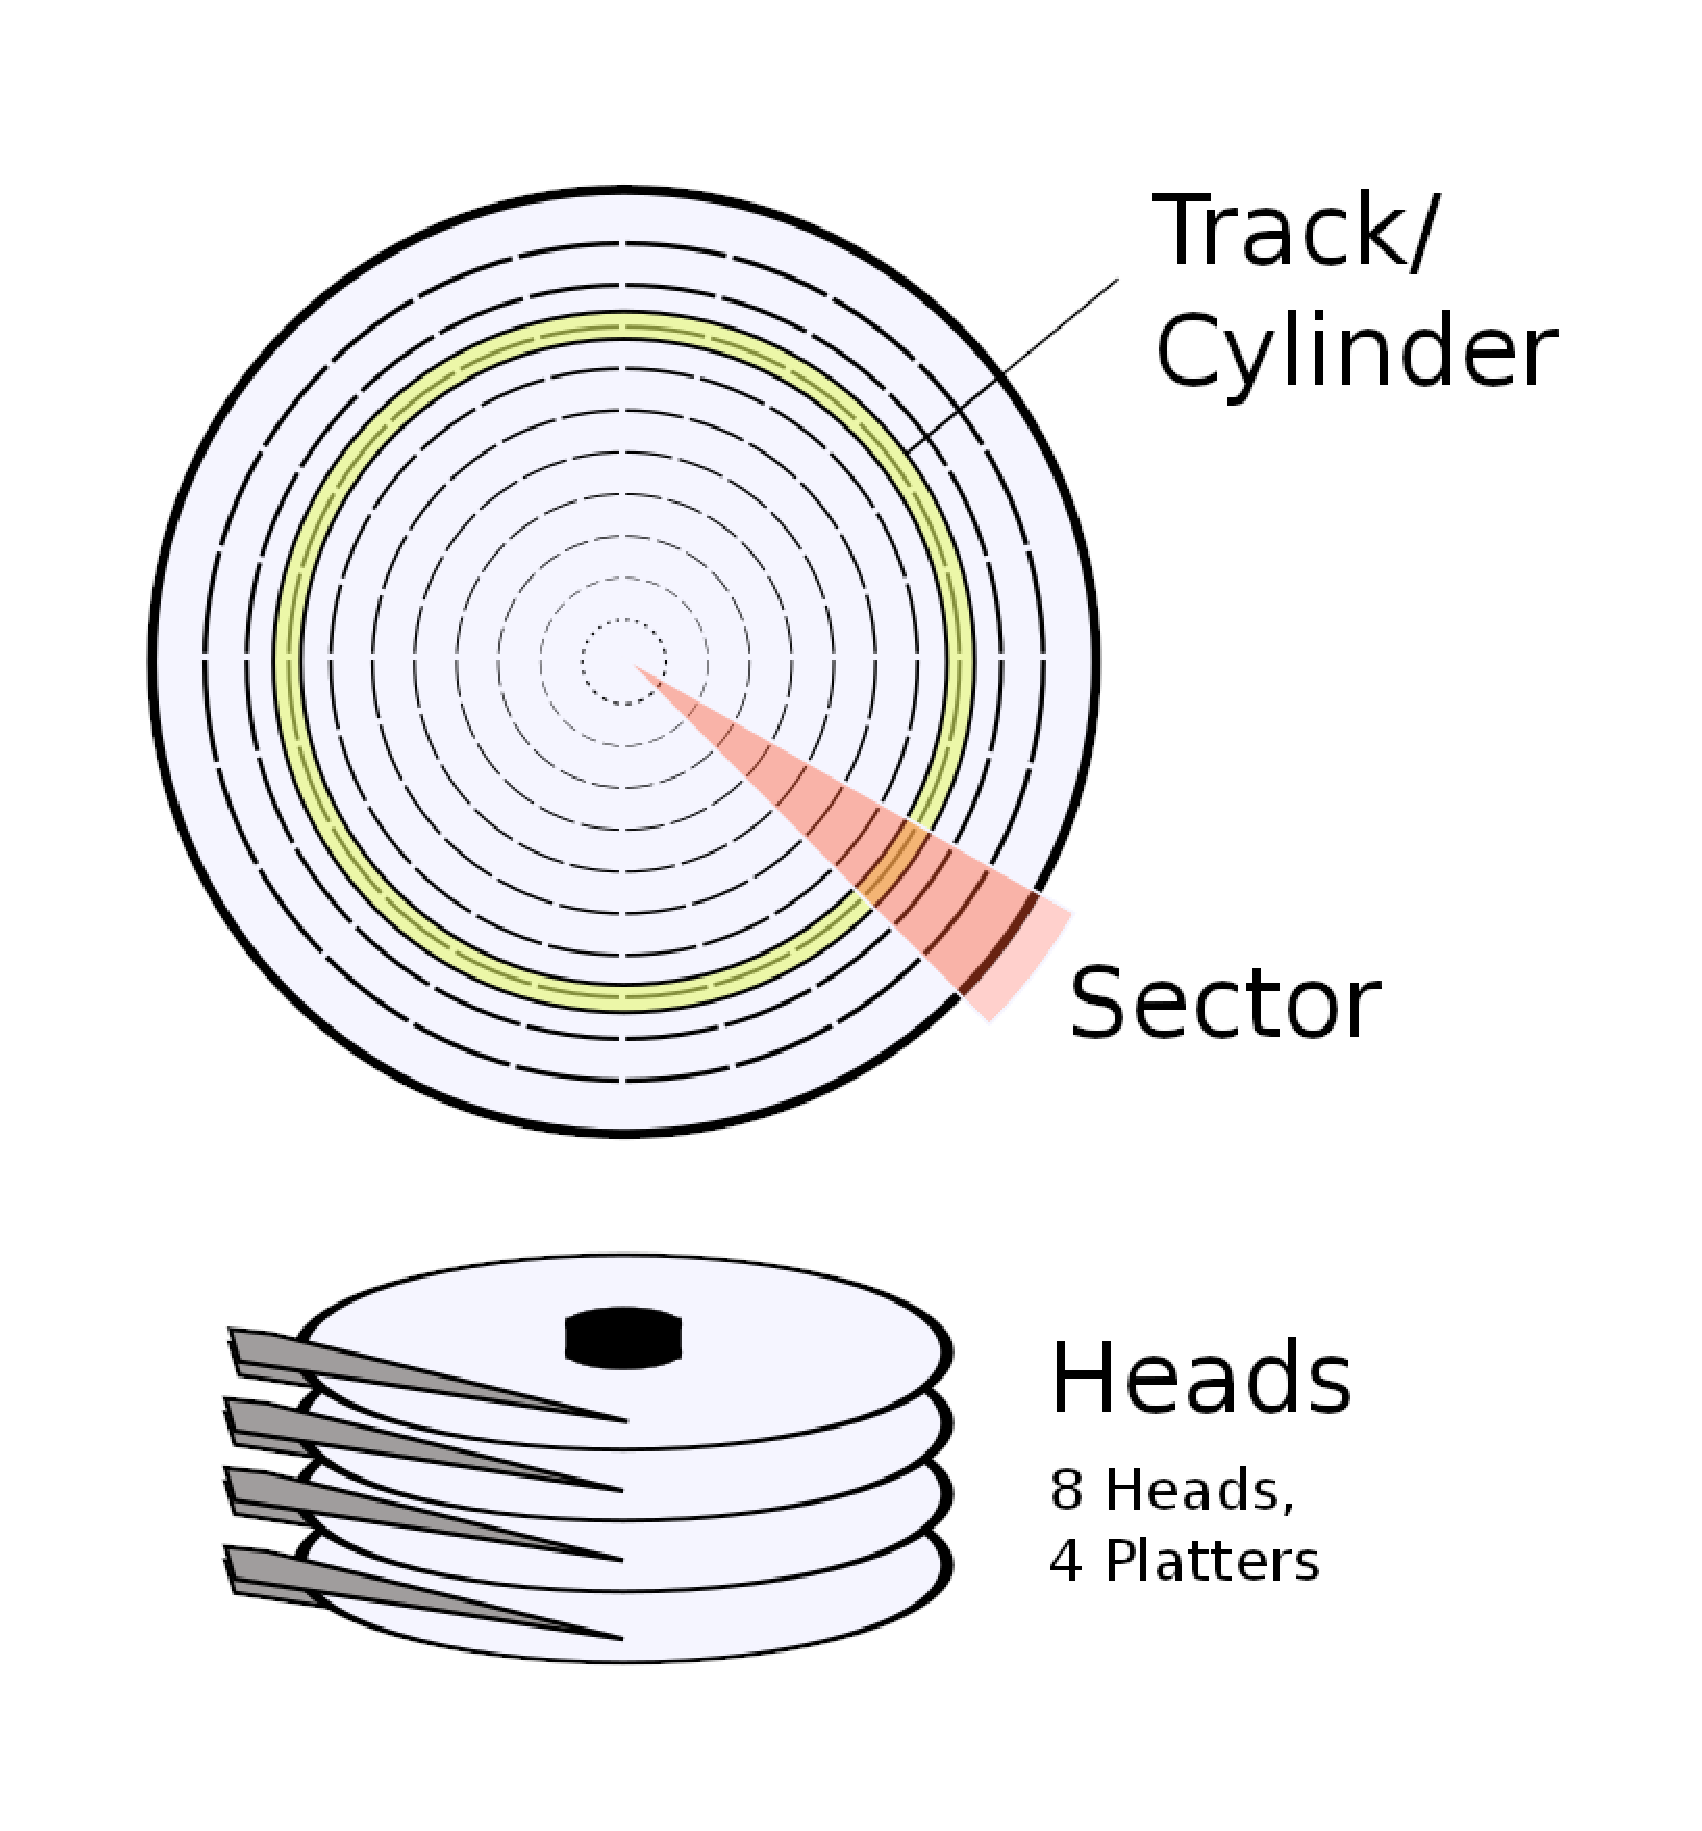
\includegraphics[scale=0.25]{figures/chs.eps}
  \caption{Cylinder/tracks, sectors and heads on a hard disk platter \cite{chsdiag}}
\label{fig:chs}
\end{figure}
For input, a standard IBM model F keyboard with 83 keys and five-pin connector was provided. The keys pressed on the keyboard were mapped to the characters present in the ROM of the CGA card. The characters present in the ROM were printable ASCII characters, diacritics, some Greek letters, and a few graphic characters. This character set present in the ROM was called IBM437 or "code page 437". Later models of IBM PC were shipped with VGA cards which supported a resolution of 640x480 pixels and had a 16-bit color palette.\\
To generate sounds, an 8254 programmable interval timer was used to generate square waves which were fed into a piezoelectric speaker.

\subsubsection{BIOS}
The term BIOS, standing for Basic I/O System, was coined by Gary Kildall. It is the firmware which is responsible for loading the bootloader from storage into the main memory. BIOS is stored in ROM and is the first software which is read by the CPU. Besides being responsible for loading the bootloader, the BIOS also provides the bootloader and real-mode OSs with several basic subroutines\footnote[1]{The words "procedure", "subroutine", and "function" have the same meaning and are used inter-changeably throughout this report.} which allow them to access the hardware.  These subroutines are called BIOS interrupts. BIOS interrupts are called by initializing the registers with appropriate values and issuing a software interrupt using \verb|int| instruction. For example, to print a character on the screen, BIOS interrupt 10,0E\footnote[1]{BIOS calls are mentioned in this report using INT N,F format. Here, N is the BIOS call number in hex-format, and F is the service which is required. F is usually an 8-bit number stored in \texttt{ah} before INT N is executed.} is used. To use this interrupt, 0x0e is stored in \texttt{ah} and the hex-code (from code page 437) of the character to be printed is stored in \texttt{al}. Then a software interrupt with interrupt number 0x10 is issued. The processor executes the ISR corresponding to interrupt 0x10 with \texttt{ah} = 0x0e in the BIOS and prints the character in \texttt{al} on the screen.\\
The BIOS in the original IBM PC was reverse engineered and cloned by other manufacturers so as to make their PCs compatible with the IBM PC. BIOS is slowly fading out of use in favour of UEFI. This is mainly because it is unsecure and is not supported in protected (32-bit) and long (64-bit) mode. \textit{Ralph Brown's Interrupt List} provides hobbyists and professionals with a comprehensive list of BIOS interrupts \cite{ralphintlist}.

\subsubsection{Boot Process}
When an IBM PC compatible computer is powered on or if the reset button is pressed, the BIOS performs a system check which is called power-on self-test (POST). POST involves initialization the main memory (RAM) and few important peripherals (e.g., keyboard, screen, speakers, disk drivers). If there is any error during POST, the BIOS informs the user about the same by generating beep codes from the speaker. Once the POST has been successfully completed, INT 19h is used to detect and load the bootloader from a bootable disk. A disk is considered to be bootable if the last word of its very first sector (track = 0 and head = 0) contains the magic number 0xaa55. As this sector also contains the bootloader, it is also known as boot sector or master boot record (MBR). Upon detecting the disk to be bootable, the BIOS loads the content of the MBR at address 0x7c00. The IP jumps to this address and CPU starts executing the instructions which make up the MBR. The bootloader might be simple enough to be contained in 512 bytes, or it might be complicated enough to be contained two sectors. In the latter scenario a two-stage bootloader is used. The boot sector code loads more sectors, and once the bootloader has been loaded, the kernel and then the operating system is loaded into the memory using BIOS calls.
\begin{figure}[h]
  \centering
  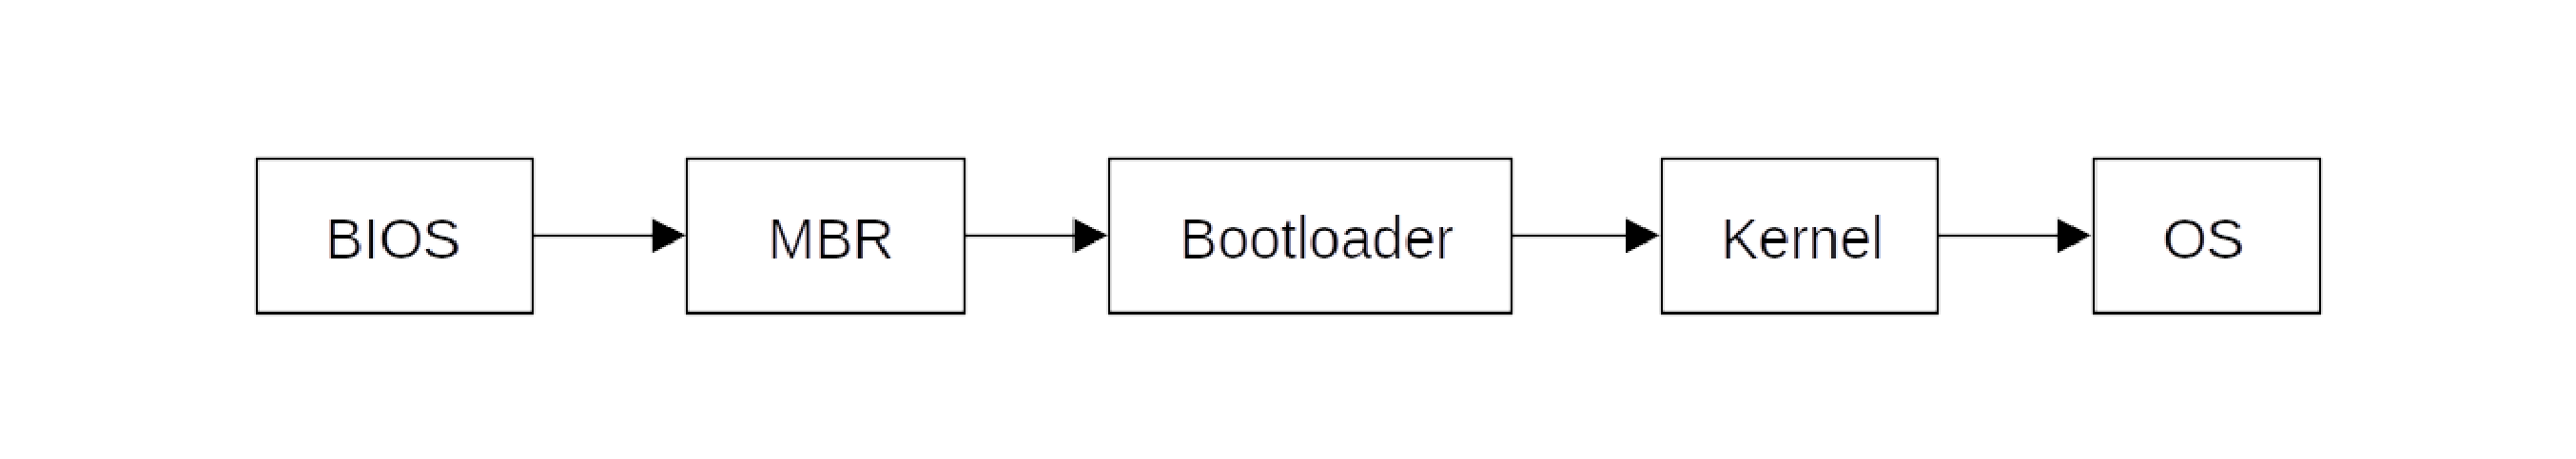
\includegraphics[scale=0.25]{figures/Booting.eps}
  \caption{Boot sequence of an IBM PC}
\label{fig:booting}
\end{figure}

\subsubsection{Memory Map}
Memory map is a diagrammatic/tabular method of showing the contents of physical memory of a computer system. In the case of the IBM PC, we are mainly interested in the memory map after booting has been completed. Therefore, by the term memory map we specifically mean the contents of memory after boot-up sequence.\\
The memory map is shown in \autoref{fig:memmap}. 

\begin{figure}[h]
  \centering
  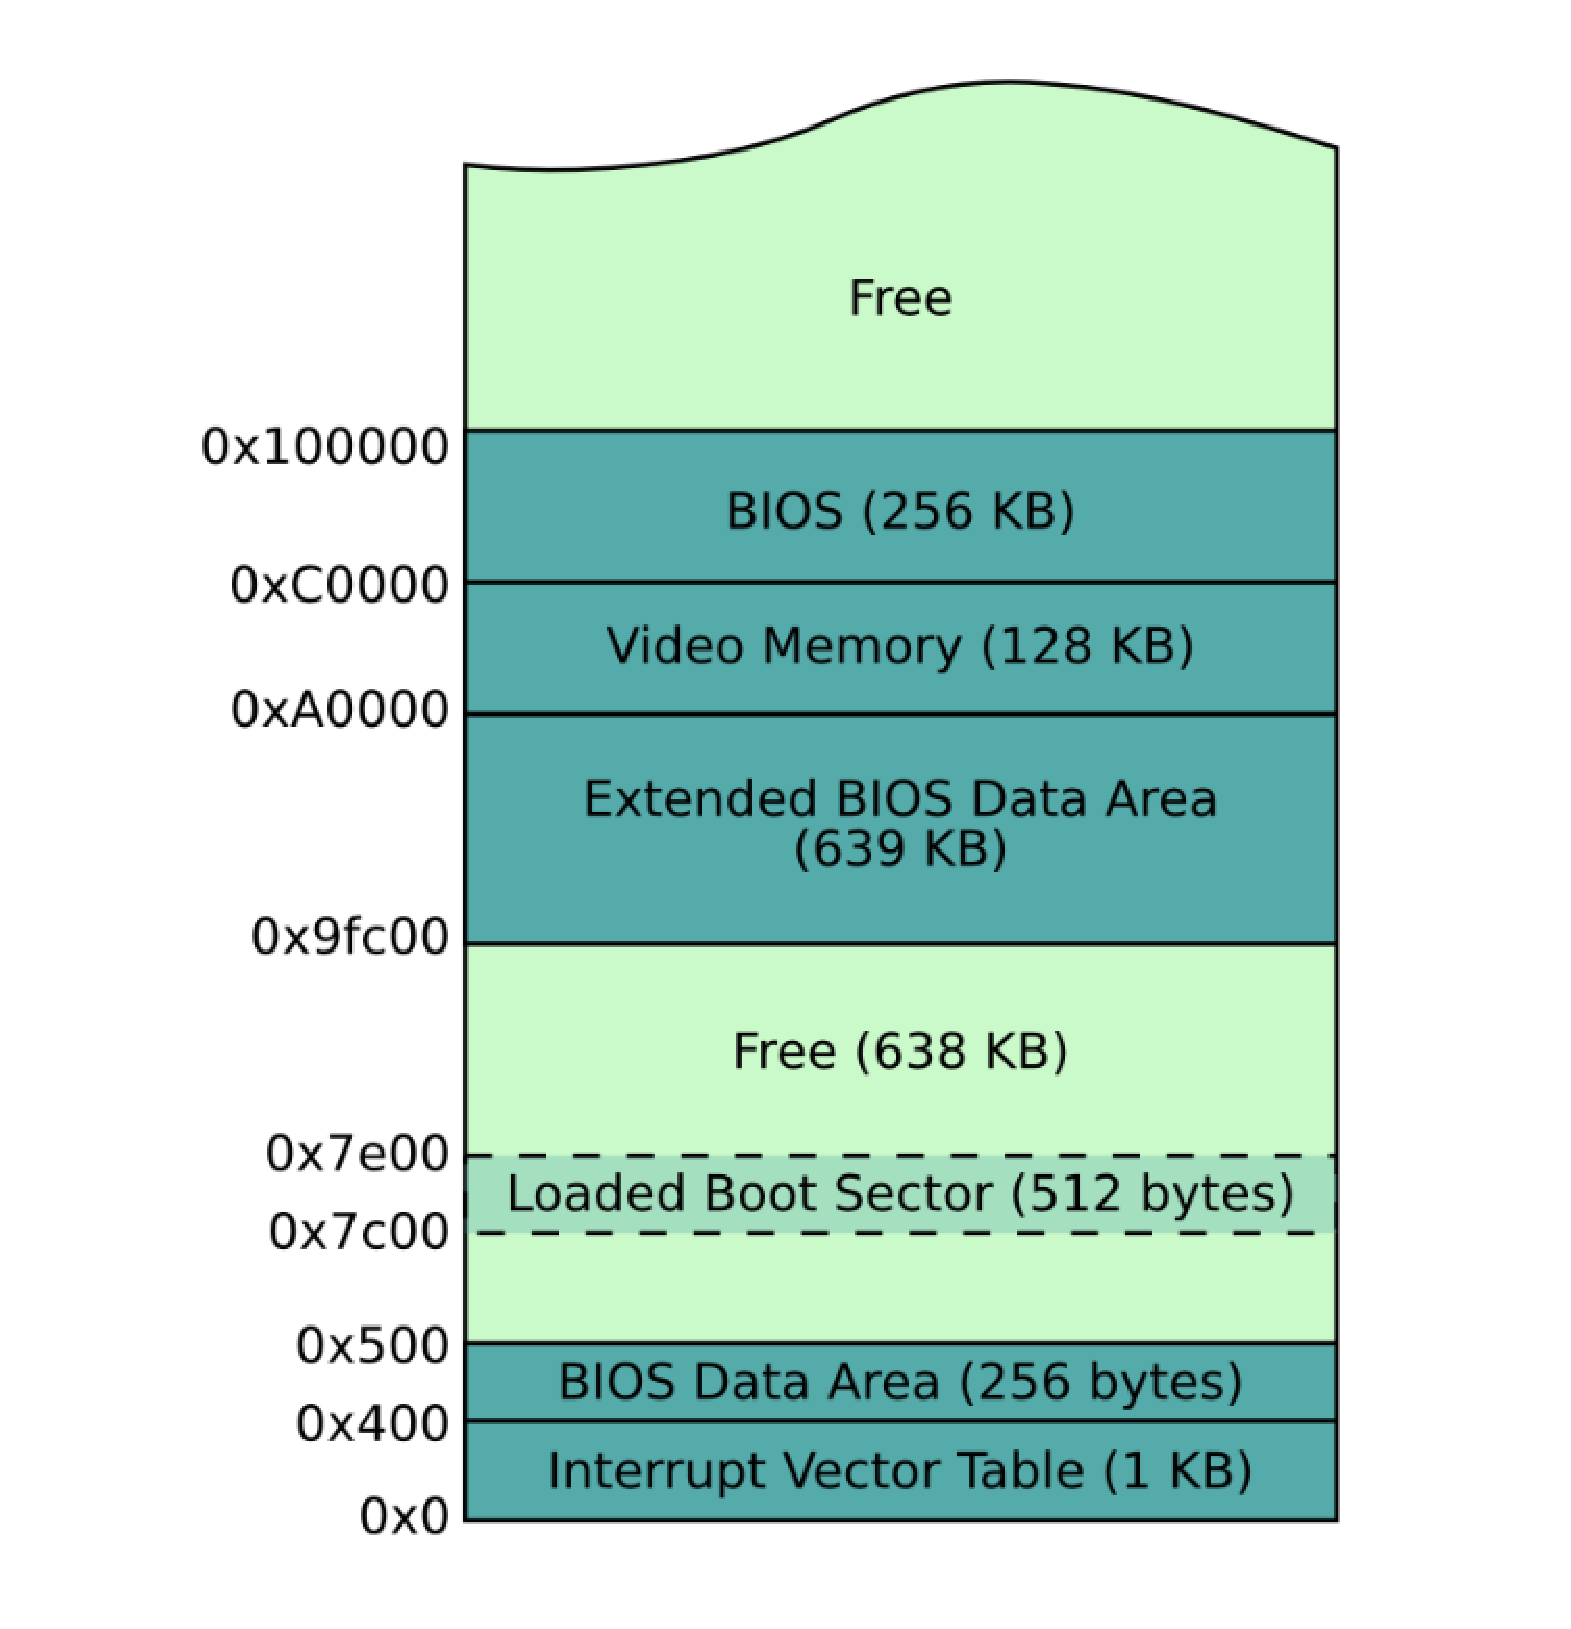
\includegraphics[scale=0.30]{figures/memmap.eps}
  \caption{Typical memory map of an IBM PC after boot \cite{blundell2009writing}}
\label{fig:memmap}
\end{figure}

As has already been discussed, the maximum size of a segment in 8086 is 64 kiB. Total addressable physical memory is 1 MiB. This memory is divided into continuous 64 kiB segments. Each of these segments is called a block. The blocks are differentiated from each other by the value of the most significant nibble of their segment base address. A block have segment base address equal to 0xn0000 is called block n. For example, the block starting at address 0x50000 is called block 5. Block 0 to block 9 make up 640 kiB of memory and together make up the \textit{low memory area} or \textit{conventional memory area} (LMA). Block A till F make up the \textit{upper memory area} (UMA) which has a size of 384 kiB. The blocks and the purpose they are usually used for is presented in \autoref{table:memmap}. Note that the blocks extended BIOS data area (EBDA) occupies varies from system to system and is, therefore, not mentioned in the table. However, EBDA is generally placed before block A.


\begin{table}[H]
\begin{center}
{\normalsize%
\caption{Typical Memory Map of an IBM PC after boot-up sequence}\label{table:memmap}
\begin{tabular}[t]{|c|c|c|c|}
\hline
\textbf{Block} & \textbf{Start} & \textbf{End} & \textbf{Description}\\
\hline
 & 0x000 & 0x3ff & Interrupt vector table (IVT)\\
	\cline{2-4}
  & 0x400 & 0x4ff & BIOS data area (BDA)\\
	\cline{2-4}
0  & 0x500 & 0x7bff & User memory\\
	\cline{2-4}
  & 0x7c00 & 0x7dff & Bootloader\\
	\cline{2-4}
  & 0x7e00 & 0xffff &\\
	\cline{1-3}
1 & 0x10000 & 0x1ffff &\\
	\cline{1-3}
2 & 0x20000 & 0x2ffff &\\
	\cline{1-3}
3 & 0x30000 & 0x3ffff &\\
	\cline{1-3}
4 & 0x40000 & 0x4ffff &\\
	\cline{1-3}
5 & 0x50000 & 0x5ffff & User memory\\
	\cline{1-3}
6 & 0x60000 & 0x6ffff &\\
	\cline{1-3}
7 & 0x70000 & 0x7ffff &\\
	\cline{1-3}
8 & 0x80000 & 0x8ffff &\\
	\cline{1-3}
9 & 0x90000 & 0x9ffff &\\
\hline
A & 0xa0000 & 0xaffff & Video memory\\
	\cline{1-3}
B & 0xb0000 & 0xbffff &\\
\hline
C & 0xc0000 & 0xcffff &\\
	\cline{1-3}
D & 0xd0000 & 0xdffff & Mapped to ROM and hardware\\
	\cline{1-3}
E & 0xe0000 & 0xeffff &\\
	\cline{1-3}
F & 0xf0000 & 0xfffff &\\
\hline
\end{tabular}}
\end{center}
\end{table}


\subsection{Deficiencies of Model Curriculum for Engineering and Technology Developed by AICTE}
We discussed in section 1.1 on how engineering is a practical profession which necessitates that engineering students should have practical knowledge of the field they establish their career in. With the aim of getting students employed in an ever-changing industry, it becomes increasingly hard to keep the syllabi appropriately updated. Neither the institutions responsible for maintaining and enforcing the curriculum, nor the students can be entirely blamed for the lack of practical knowledge which can be found among many freshers across the globe. A discussion of the global technical education scenario would increase the length of the present chapter which is already beyond the usual length. Therefore, we will restrict our discussion to the brief analysis of engineering education in India. This will be appropriate as:
\begin{enumerate}
\item All the authors of this report bear the nationality of Indian.
\item It is estimated that India will be the leading producers of engineers by the end of the current and the coming decades \cite{ind2015eng}. This makes it important that the quality of engineers being produced is great.
\end{enumerate}
It is a well known fact that engineering education in India is not at par with the requirements of the industry. This fact has been pointed out by many people over the years, more recently by Steve Wozniak who pointed out that innovation has taken a backseat in pursuit of employability \cite{woz2018eng}. Such criticism often results in a blame game. Sometimes counterarguments also blame the British rule. The fact that after more than half a century of independence, we, as a nation, have failed to nurture and promote original thinking and creativity is disregarded. The number of jobs related to computer science and IT are ever increasing. Students in pursuit of getting employed often curb their interests and enrol in courses related to computer science and IT \cite{popengtoi}. Innovation and practicality go hand in hand. The saying "\textit{Necessity is the mother of innovation}" is an adage to this. Without getting their hands dirty, a person can never know about the requirements of a particular field. Therefore, it becomes necessary to ensure that students are dispensed practical knowledge in as many areas as possible. By doing so, they can determine their interests and contribute to the fields they like. The best way to dispense practical knowledge is by incorporating project-based learning in the curriculum for technical education.\\
Though the model curriculum provided by the All India Council for Technical Education (AICTE) is developed with the help of academic and industry experts \cite{basu2018model}, they have some glaring flaws, three of which are stated below.
\begin{enumerate}
	\item \textit{Undirected and overloaded course structure}: A single course consists of many theoretical sub-topics without any practical problems for students to work through. A student can solve tons of problems on Kirchhoff's rules however their ability to synthesize a circuit is equally important. As the project presented in this report is related to computer architecture and operating systems, we will take the example the course on Computer Architecture offered to Electrical Engineering undergrads. There are six modules in this course. Module 1 tells about the differences between CISC and RISC, data types, system buses, and multi-bus organization. Module 2 then jumps to memory organization, followed by Module 3 discussing I/O devices, PCI and PCI Express bus. Module 4 then discusses x86 architecture, and its addressing modes and instruction. Module 5 discusses instruction level pipelining (ILP) and module 6 discusses other architectures like MIPS. The course, and other similar courses, can be considered to be well designed theoretically. However, they are overloaded with theoretical concepts. It would be better to just focus on the architecture of single computer, preferably IBM PC. The course can then describe the 8086 microprocessor and later describe ILP, and paging. Then the architecture of the IBM PC can be dealt with in detail.
	\item \textit{Impractical course structure}: Continuing with the example provided previously, most of the courses dealing with microprocessors start of with 8085 microprocessor. Though it is still used in legacy systems in the industry, no new projects are developed using it. Students would be better served by teaching them about ARM or RISC-V or x86 architectures as most of the computing systems today are built around them. Furthermore, it must be noted that the practical assignments given to students are trivial. Examples include writing subroutines to multiply numbers, or to move strings in 8086's assembly language. A more practical exercise would be to write subroutines to print a string on the screen or to separate words out from a string.   
	\item \textit{Obsolete software tools}: Most of the software tools used in colleges are obsolete. Courses on C programming and data structures still require students to develop and run code in Turbo C environment. This is ridiculous because Turbo C's compiler does not follow the standard implementation of C and C++. In the course on microprocessors, codes are run on expensive trainer kits or on emulators, like emu8086, which is not the industry standard for developing 8086 assembly code.
\end{enumerate}
Remedying the current problems will take years. However, one should not be daunted by this challenge. Baby-steps are what is required. The project presented in this report is one such baby-step. It is hoped that it will assist in nurturing students who are interested in computer architecture and they will not have to face the problems which the author of this project (Kapoor) had to face.

